%
% Template Laporan Skripsi/Thesis 
%
% @author  Andreas Febrian, Lia Sadita 
% @version 1.03
%
% Dokumen ini dibuat berdasarkan standar IEEE dalam membuat class untuk 
% LaTeX dan konfigurasi LaTeX yang digunakan Fahrurrozi Rahman ketika 
% membuat laporan skripsi. Konfigurasi yang lama telah disesuaikan dengan 
% aturan penulisan thesis yang dikeluarkan UI pada tahun 2008.
%

%
% Tipe dokumen adalah report dengan satu kolom. 
%
\documentclass[12pt, a4paper, onecolumn, oneside, final]{report}

% Load konfigurasi LaTeX untuk tipe laporan thesis
\usepackage{url}
\usepackage{uithesis}

\usepackage{listings}
\usepackage{courier}
\usepackage{color}
\definecolor{sh_comment}{rgb}{0.12, 0.38, 0.18 } %adjusted, in Eclipse: {0.25, 0.42, 0.30 } = #3F6A4D
\definecolor{sh_keyword}{rgb}{0.37, 0.08, 0.25}  % #5F1441
\definecolor{sh_string}{rgb}{0.06, 0.10, 0.98} % #101AF9
\usepackage{xcolor}
\usepackage{caption}
\DeclareCaptionFont{white}{\color{white}}
\DeclareCaptionFormat{listing}{%
	\parbox{\textwidth}{\colorbox{gray}{\parbox{\textwidth}{#1#2#3}}\vskip-4pt}}
\captionsetup[lstlisting]{format=listing,labelfont=white,textfont=white}
\lstset{frame=lrb,xleftmargin=\fboxsep,xrightmargin=-\fboxsep}
\renewcommand{\lstlistingname}{Kode}
\usepackage{courier}
\lstset {
	rulesepcolor=\color{black},
	showspaces=false,showtabs=false,tabsize=2,
	numberstyle=\tiny,numbers=left,
	basicstyle=\footnotesize\ttfamily\bfseries,
	stringstyle=\color{sh_string},
	keywordstyle = \color{sh_keyword}\bfseries,
	commentstyle=\color{sh_comment}\itshape,
	breaklines=true
}

\usepackage[backend=bibtex,style=numeric]{biblatex}
\bibliography{referensi}


% Load konfigurasi khusus untuk laporan yang sedang dibuat
%-----------------------------------------------------------------------------%
% Informasi Mengenai Dokumen
%-----------------------------------------------------------------------------%
% 
% Judul laporan. 
\var{\judul}{Judul Skripsi/Thesis/Disertasi}
% 
% Tulis kembali judul laporan, kali ini akan diubah menjadi huruf kapital
\Var{\Judul}{Judul Skripsi/Thesis/Disertasi}
% 
% Tulis kembali judul laporan namun dengan bahasa Ingris
\var{\judulInggris}{Unknown Title for Final Report/Thesis/Disertation}

% 
% Tipe laporan, dapat berisi Skripsi, Tugas Akhir, Thesis, atau Disertasi
\var{\type}{Tugas Akhir}
% 
% Tulis kembali tipe laporan, kali ini akan diubah menjadi huruf kapital
\Var{\Type}{Tugas Akhir}
% 
% Tulis nama penulis 
\var{\penulis}{Luqman Sungkar}
% 
% Tulis kembali nama penulis, kali ini akan diubah menjadi huruf kapital
\Var{\Penulis}{Luqman Sungkar}
% 
% Tulis NPM penulis
\var{\npm}{1106088303}
% 
% Tuliskan Fakultas dimana penulis berada
\Var{\Fakultas}{Fakultas Ilmu Komputer}
\var{\fakultas}{Fakultas Ilmu Komputer}
% 
% Tuliskan Program Studi yang diambil penulis
\Var{\Program}{Sistem Informasi}
\var{\program}{Sistem Informasi}
% 
% Tuliskan tahun publikasi laporan
\Var{\bulanTahun}{Januari 2010}
% 
% Tuliskan gelar yang akan diperoleh dengan menyerahkan laporan ini
\var{\gelar}{Sarjana Ilmu Komputer}
% 
% Tuliskan tanggal pengesahan laporan, waktu dimana laporan diserahkan ke 
% penguji/sekretariat
\var{\tanggalPengesahan}{XX Januari 2010} 
% 
% Tuliskan tanggal keputusan sidang dikeluarkan dan penulis dinyatakan 
% lulus/tidak lulus
\var{\tanggalLulus}{XX Januari 2010}
% 
% Tuliskan pembimbing 
\var{\pembimbing}{Prof. XXXX}
% 
% Alias untuk memudahkan alur penulisan paa saat menulis laporan
\var{\saya}{Penulis}
\var{\iot}{\textit{internet of things}}
\var{\IOT}{Internet of Things}
\var{\eu}{\textit{end-user}}
\var{\plat}{\textit{platform}}
\var{\siot}{\textit{social internet of things}}
\var{\gateway}{\textit{gateway}}
\var{\Gateway}{\textit{Gateway}}

%-----------------------------------------------------------------------------%
% Judul Setiap Bab
%-----------------------------------------------------------------------------%
% 
% Berikut ada judul-judul setiap bab. 
% Silahkan diubah sesuai dengan kebutuhan. 
% 
\Var{\kataPengantar}{Kata Pengantar}
\Var{\babSatu}{Pendahuluan}
\Var{\babDua}{Landasan Teori}
\Var{\babTiga}{Rancangan Implementasi}
\Var{\babEmpat}{Implementasi}
\Var{\babLima}{Pengujian}
\Var{\babEnam}{??}
\Var{\kesimpulan}{Kesimpulan dan Saran}

% Daftar pemenggalan suku kata dan istilah dalam LaTeX
%
% Hyphenation untuk Indonesia 
%
% @author  Andreas Febrian
% @version 1.00
% 
% Tambahkan cara pemenggalan kata-kata yang salah dipenggal secara otomatis 
% oleh LaTeX. Jika kata tersebut dapat dipenggal dengan benar, maka tidak 
% perlu ditambahkan dalam berkas ini. Tanda pemenggalan kata menggunakan 
% tanda '-'; contoh:
% menarik
%   --> pemenggalan: me-na-rik
%

\hyphenation{
    % alphabhet A
    a-na-li-sa a-tur 
    a-pli-ka-si 
    automation
    % alphabhet B
    ba-ngun-an 
    be-be-ra-pa 
    ber-ge-rak
    ber-ke-lan-jut-an 
    ber-pe-nga-ruh 
    berbasis
    berbasiskan
    % alphabhet C
    ca-ri
    coordinator
    % alphabhet D
    di-sim-pan di-pim-pin de-ngan da-e-rah di-ba-ngun da-pat di-nya-ta-kan 
    di-sim-bol-kan di-pi-lih di-li-hat de-fi-ni-si
    dimiliki
    % alphabhet E
    e-ner-gi eks-klu-sif
    % alphabhet F
    fa-si-li-tas
    % alphabhet G
    ga-bung-an ge-rak
    % alphabhet H
    ha-lang-an
    % alphabhet I
    implementasi
    % alphabhet J
    % alphabhet K
    ke-hi-lang-an
    ku-ning 
    kua-li-tas ka-me-ra ke-mung-kin-an ke-se-pa-ham-an
    konsep
    % alphabhet L
    ling-kung-an
    % alphabhet M
    me-neng-ah
    meng-a-tas-i me-mung-kin-kan me-nge-na-i me-ngi-rim-kan 
    meng-u-bah meng-a-dap-ta-si me-nya-ta-kan mo-di-fi-ka-si
    meng-a-tur
    miliki
    % alphabhet N
    nya-ta non-eks-klu-sif
    % alphabhet O
    % alphabhet P
	pe-nye-rap-an 
	pe-ngon-trol
    pe-mo-del-an
    pe-ran  pe-ran-an-nya
    pem-ba-ngun-an pre-si-den pe-me-rin-tah prio-ri-tas peng-am-bil-an 
    peng-ga-bung-an pe-nga-was-an pe-ngem-bang-an 
    pe-nga-ruh pa-ra-lel-is-me per-hi-tung-an per-ma-sa-lah-an 
    pen-ca-ri-an peng-struk-tur-an
    platform
    perintah
    pengelola
    % alphabhet Q
    % alphabhet R
    ran-cang-an
    % alphabhet S
    si-mu-la-si sa-ngat
    % alphabhet T
    te-ngah
    ter-da-pat
    tujuan
    tahapan
    % alphabhet U
    % alphabhet V
    % alphabhet W
    % alphabhet X
    % alphabhet Y
    % alphabhet Z
    % special
}
% Daftar istilah yang mungkin perlu ditandai 
%
% @author  Andreas Febrian
% @version 1.00
% 
% Mendaftar seluruh istilah yang mungkin akan perlu dijadikan 
% italic atau bold pada setiap kemunculannya dalam dokumen. 
% 

\var{\license}{\f{Creative Common License 1.0 Generic}}
\var{\bslash}{$\setminus$}

% Awal bagian penulisan laporan
\begin{document}
%
% Sampul Laporan
%
% Sampul Laporan

%
% @author  unknown
% @version 1.01
% @edit by Andreas Febrian
%

\begin{titlepage}
    \begin{center}    
        \begin{figure}
            \begin{center}
                
\includegraphics[width=2.5cm]{pics/makara.png}
            \end{center}
        \end{figure}    
        \vspace*{0cm}
        \bo{
        	UNIVERSITAS INDONESIA\\
        }
        
        \vspace*{1.0cm}
        % judul thesis harus dalam 14pt Times New Roman
        \bo{\Judul} \\[1.0cm]

        \vspace*{2.5 cm}    
        % harus dalam 14pt Times New Roman
        \bo{\Type}

        \vspace*{3 cm}       
        % penulis dan npm
        \bo{\Penulis} \\
        \bo{\npm} \\

        \vspace*{5.0cm}

        % informasi mengenai fakultas dan program studi
        \bo{
        	FAKULTAS \Fakultas\\
        	PROGRAM STUDI \Program \\
        	DEPOK \\
        	\bulanTahun
        }
    \end{center}
\end{titlepage}


%
% Gunakan penomeran romawi
\pagenumbering{roman}

%
% load halaman judul dalam
\addChapter{HALAMAN JUDUL}
%
% Halaman Judul Laporan 
%
% @author  unknown
% @version 1.01
% @edit by Andreas Febrian
%

\begin{titlepage}
    \begin{center}\begin{figure}
            \begin{center}
                
\includegraphics[width=2.5cm]{pics/makara.png}
            \end{center}
        \end{figure}    
        \vspace*{0cm}
        \bo{
        	UNIVERSITAS INDONESIA\\
        }
        
        \vspace*{1.0cm}
        % judul thesis harus dalam 14pt Times New Roman
        \bo{\Judul} \\[1.0cm]

        \vspace*{2.5 cm}    
        % harus dalam 14pt Times New Roman
        \bo{\Type} \\
        % keterangan prasyarat
        \bo{Diajukan sebagai salah satu syarat untuk memperoleh gelar \\
        \gelar}\\

        \vspace*{3 cm}       
        % penulis dan npm
        \bo{\Penulis} \\
        \bo{\npm} \\

        \vspace*{5.0cm}

        % informasi mengenai fakultas dan program studi
        \bo{
        	FAKULTAS \Fakultas\\
        	PROGRAM STUDI \Program \\
        	DEPOK \\
        	\bulanTahun
        }
    \end{center}
\end{titlepage}

%
% setelah bagian ini, halaman dihitung sebagai halaman ke 2
\setcounter{page}{2}

%
% load halaman pengesahan
\addChapter{LEMBAR PERSETUJUAN}
%
% Halaman Pengesahan
%
% @author  Andreas Febrian
% @version 1.01
%

\chapter*{HALAMAN PERSETUJUAN}

\vspace*{0.2cm}
\noindent 

\noindent
\begin{tabular}{l l p{11cm}}
	\bo{Judul}&: & \judul \\ 
	\bo{Nama}&: & \penulis \\
	\bo{NPM}&: & \npm \\
\end{tabular} \\

\vspace*{1.2cm}

\noindent Laporan \type~ini telah diperiksa dan disetujui.\\[0.3cm]
\begin{center}
\tanggalPengesahan \\[2cm]


\underline{\pembimbing}\\[0.1cm]
Pembimbing \type
\end{center}

\newpage
%
% load halaman orisinalitas 
\addChapter{LEMBAR PERNYATAAN ORISINALITAS}
%
% Halaman Orisinalitas
%
% @author  Andreas Febrian
% @version 1.01
%

\chapter*{\uppercase{halaman pernyataan orisinalitas}}
\vspace*{2cm}

\begin{center}
	\bo{\type~ini adalah hasil karya saya sendiri, \\ 
	dan semua sumber baik yang dikutip maupun dirujuk \\
	telah saya nyatakan dengan benar.} \\
	\vspace*{2.6cm}
	
	\begin{tabular}{l c l}
	\bo{Nama} & : & \bo{\penulis} \\
	\bo{NPM} & : & \bo{\npm} \\ 
	\bo{Tanda Tangan} & : & \\
	& & \\
	& & \\
	\bo{Tanggal} & : & \bo{\tanggalPengesahan} \\	
	\end{tabular}
\end{center}

\newpage
%
%
\addChapter{LEMBAR PENGESAHAN}
%
% Halaman Pengesahan Sidang
%
% @author  Andreas Febrian, Andre Tampubolon 
% @version 1.02
%

\chapter*{HALAMAN PENGESAHAN}

\vspace*{0.4cm}
\noindent 

\noindent
\begin{tabular}{ll p{9cm}}
	\type~ini diajukan oleh&: & \\
	Nama&: & \penulis \\
	NPM&: & \npm \\
	Program Studi&: & \program \\
	Judul \type&: & \judul \\
\end{tabular} \\

\vspace*{1.0cm}

\noindent \bo{Telah berhasil dipertahankan di hadapan Dewan Penguji 
dan diterima sebagai bagian persyaratan yang diperlukan untuk 
memperoleh gelar \gelar~pada Program Studi \program, Fakultas 
\fakultas, Universitas Indonesia.}\\[0.2cm]

\begin{center}
	\bo{DEWAN PENGUJI}
\end{center}

\vspace*{0.3cm}

\begin{tabular}{l l l l }
	& & & \\
	Pembimbing&: & \pembimbing & (\hspace*{3.0cm}) \\
	& & & \\
	Penguji&: & Prof. XXX & (\hspace*{3.0cm}) \\
	& & & \\
	Penguji&: & Prof. XXXX & (\hspace*{3.0cm}) \\
	& & & \\
	Penguji&: & Prof. XXXXXX & (\hspace*{3.0cm}) \\
\end{tabular}\\


\vspace*{2.0cm}

\begin{tabular}{ll l}
	Ditetapkan di&: & Depok\\
	Tanggal&: & \tanggalLulus \\
\end{tabular}


\newpage
%
%
\addChapter{\kataPengantar}
%-----------------------------------------------------------------------------%
\chapter*{\kataPengantar}
%-----------------------------------------------------------------------------%
Template ini disediakan untuk orang-orang yang berencana menggunakan 
\latex~untuk membuat dokumen tugas akhirnya. 
Mengapa \latex? 
Ada banyak hal mengapa menggunakan \latex, diantaranya:

\begin{enumerate}
	\item \latex~membuat kita jadi lebih fokus terhadap isi dokumen, bukan 
		tampilan atau halaman. 
	\item \latex~memudahkan dalam penulisan persamaan matematis. 
	\item Adanya automatis dalam penomoran caption, bab, subbab, subsubbab, 
		referensi, dan rumus. 
	\item Adanya automatisasi dalam pembuatan daftar isi, daftar gambar, dan
		daftar tabel. 
	\item Adanya kemudahan dalam memberikan referensi dalam tulisan dengan 
		menggunakan label. Cara ini dapat meminimalkan kesalahan pemberian 
		referensi. 
\end{enumerate}

Template ini bebas digunakan dan 
didistribusikan sesuai dengan aturan \license, yang secara sederhana berisi: 

\begin{figure}
	\centering
	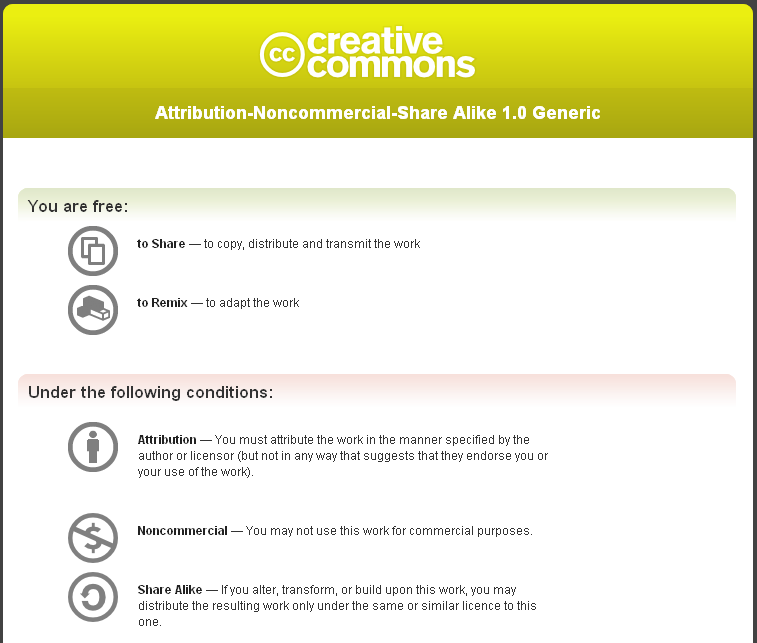
\includegraphics[width=0.74\textwidth]
		{pics/creative_common.png}
	\caption{\license}
	\label{fig:lisensi}
\end{figure}

\pic~\ref{fig:lisensi} diambil dari 
\url{http://creativecommons.org/licenses/by-nc-sa/1.0/deed.en_CA}. 
Jika ingin mengentahui lebih lengkap mengenai \license, silahkan buka 
\url{http://creativecommons.org/licenses/by-nc-sa/1.0/legalcode}. 
Seluruh dokumen yang dibuat dengan menggunakan template ini sepenuhnya 
menjadi hak milik pembuat dokumen dan bebas didistribusikan sesuai dengan 
keperluan masing-masing. 
Lisensi hanya berlaku jika ada orang yang membuat template baru dengan 
menggunakan template ini sebagai dasarnya. 

Dokumen ini dibuat dengan \latex~juga. Untuk meyakinkan Anda, coba lihat 
properti dari dokumen ini dan Anda akan menemukan bagian seperti 
\pic~\ref{fig:pdflatex}. 
Dokumen ini dimaksudkan untuk memberikan gambaran kepada Anda seperti apa 
mudahnya menggunakan \latex~dan juga memperlihatkan betapa bagus dokumen 
yang dihasilkan. 
Seluruh url yang Anda temukan dapat Anda klik. 
Seluruh referensi yang ada juga dapat diklik. 
Untuk mengerti template yang disediakan, Anda tetap harus membuka kode 
\latex~dan bermain-main dengannya. 
Penjelasan dalam PDF ini masih bersifat gambaran dan tidak begitu 
mendetail, dapat dianggap sebagai pengantar singkat. 
Jika Anda merasa kesulitan dengan template ini, mungkin ada baiknya 
Anda belajar sedikit dasar-dasar \latex. 

\begin{figure}
	\centering
	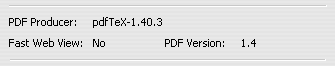
\includegraphics[width=0.54\textwidth]
		{pics/mark.png}
	\caption{Dokumen Dibuat dengan PDFLatex}
	\label{fig:pdflatex}
\end{figure}

Semoga template ini dapat membantu orang-orang yang ingin mencoba menggunakan 
\latex. Semoga template ini juga tidak berhenti disini dengan ada kontribusi 
dari para penggunanya. 
Kami juga ingin berterima kasih kepada Andreas Febrian, Lia Sadita, Fahrurrozi 
Rahman, Andre Tampubolon, dan Erik Dominikus atas kontribusinya dalam template 
ini. 

\vspace*{0.1cm}
\begin{flushright}
Depok, 30 Desember 2009\\[0.1cm]
\vspace*{1cm}
\penulis

\end{flushright}
%
%
\addChapter{LEMBAR PERSETUJUAN PUBLIKASI ILMIAH}
% 
% @author  Andre Tampubolon, Andreas Febrian
% @version 1.01
% 

\chapter*{\uppercase{Halaman Pernyataan Persetujuan Publikasi Tugas Akhir untuk Kepentingan Akademis}}

\vspace*{0.2cm}
\noindent 
Sebagai sivitas akademik Universitas Indonesia, saya yang bertanda 
tangan di bawah ini:
\vspace*{0.4cm}


\begin{tabular}{p{4.2cm} l p{6cm}}
	\bo{Nama} & : & \penulis \\ 	
	\bo{NPM} & : & \npm \\
	\bo{Program Studi} & : & \program\\	
	\bo{Fakultas} & : & \fakultas\\
	\bo{Jenis Karya} & : & \type \\
\end{tabular}

\vspace*{0.6cm}
\noindent demi pengembangan ilmu pengetahuan, menyetujui untuk memberikan 
kepada Universitas Indonesia \bo{Hak Bebas Royalti Noneksklusif 
(Non-exclusive Royalty Free Right)} atas karya ilmiah saya yang berjudul:
\begin{center}
	\judul
\end{center}
beserta perangkat yang ada (jika diperlukan). Dengan Hak Bebas Royalti 
Noneksklusif ini Universitas Indonesia berhak menyimpan, 
mengalihmedia/formatkan, mengelola dalam bentuk pangkalan data 
(database), merawat, dan memublikasikan tugas akhir saya selama 
tetap mencantumkan nama saya sebagai penulis/pencipta dan sebagai 
pemilik Hak Cipta. \\

\noindent Demikian pernyatan ini saya buat dengan sebenarnya.

\begin{center}
	\vspace*{0.8cm}
	\begin{tabular}{lll}
		Dibuat di&: & Depok \\
		Pada tanggal&: & \tanggalPengesahan \\
	\end{tabular}\\

	\vspace*{0.2cm}
	Yang menyatakan \\
	\vspace*{1.1cm}
	(\penulis)
\end{center}

\newpage


%
% 
\addChapter{ABSTRAK}
%
% Halaman Abstrak
%
% @author  Andreas Febrian
% @version 1.00
%

\chapter*{Abstrak}

\vspace*{0.2cm}

\noindent \begin{tabular}{l l p{10cm}}
	Nama&: & \penulis \\
	Program Studi&: & \program \\
	Judul&: & \judul \\
\end{tabular} \\ 

\vspace*{0.5cm}

\noindent \todo{Tuliskan abstrak laporan disini.} \\

\vspace*{0.2cm}

\noindent Kata Kunci: \\ 
\noindent \todo{Tuliskan kata kunci yang berhubungan dengan laporan 
	disini} \\

\newpage
%
%
%
% Halaman Abstract
%
% @author  Andreas Febrian
% @version 1.00
%

\chapter*{ABSTRACT}

\vspace*{0.2cm}

\noindent \begin{tabular}{l l p{11.0cm}}
	Name&: & \penulis \\
	Program&: & \program \\
	Title&: & \judulInggris \\
\end{tabular} \\ 

\vspace*{0.5cm}

\noindent \todo{Write your abstract here.}\\

\vspace*{0.2cm}

\noindent Keywords: \\ 
\noindent \todo{Write up keywords about your report here.}

\newpage

%
% Daftar isi, gambar, dan tabel
%
\tableofcontents
\clearpage
\listoffigures
\clearpage
\listoftables
\clearpage

%
% Gunakan penomeran Arab (1, 2, 3, ...) setelah bagian ini.
%
\pagenumbering{arabic}

%
%
%
%-----------------------------------------------------------------------------%
\chapter{\babSatu}
%-----------------------------------------------------------------------------%
Pada bagian ini akan dijelaskan latar belakang dari pengerjaan tugas akhir ini, tujuan penulisan, rumusan masalah, ruang lingkup dan batasan pengerjaan, tahapan pengerjaan, dan sistematika penulisan laporan.


%-----------------------------------------------------------------------------%
\section{Latar Belakang}
%-----------------------------------------------------------------------------%
\todo{tuliskan latar belakang penelitian disini}


%-----------------------------------------------------------------------------%
\section{Permasalahan}
%-----------------------------------------------------------------------------%
Pada bagian ini akan dijelaskan mengenai definisi permasalahan 
yang \saya~hadapi dan ingin diselesaikan serta asumsi dan batasan 
yang digunakan dalam menyelesaikannya.


%-----------------------------------------------------------------------------%
\subsection{Definisi Permasalahan}
%-----------------------------------------------------------------------------%
\todo{Tuliskan permasalahan yang ingin diselesaikan. Bisa juga
	berbentuk pertanyaan}


%-----------------------------------------------------------------------------%
\subsection{Batasan Permasalahan}
%-----------------------------------------------------------------------------%
\todo{Umumnya ada asumsi atau batasan yang digunakan untuk 
	menjawab pertanyaan-pertanyaan penelitian diatas.}


%-----------------------------------------------------------------------------%
\section{Tujuan}
%-----------------------------------------------------------------------------%
\todo{Tuliskan tujuan penelitian.}


%-----------------------------------------------------------------------------%
\section{Posisi Penelitian}
%-----------------------------------------------------------------------------%
\todo{Posisi penelitian Anda jika dilihat secara bersamaan dengan 
	peneliti-peneliti lainnya. Akan lebih baik lagi jika ikut menyertakan 
	diagram yang menjelaskan hubungan dan keterkaitan antar 
	penelitian-penelitian sebelumnya}


%-----------------------------------------------------------------------------%
\section{Metodologi Penelitian}
%-----------------------------------------------------------------------------%
\todo{Tuliskan metodologi penelitian yang digunakan.}


%-----------------------------------------------------------------------------%
\section{Sistematika Penulisan}
%-----------------------------------------------------------------------------%
Sistematika penulisan laporan adalah sebagai berikut:
\begin{itemize}
	\item Bab 1 \babSatu \\
	\item Bab 2 \babDua \\
	\item Bab 3 \babTiga \\
	\item Bab 4 \babEmpat \\
	\item Bab 5 \babLima \\
	\item Bab 6 \babEnam \\
	\item Bab 7 \kesimpulan \\
\end{itemize}

\todo{Tambahkan penjelasan singkat mengenai isi masing-masing bab.}


%-----------------------------------------------------------------------------%
\chapter{\babDua}
%-----------------------------------------------------------------------------%
\todo{tambahkan kata-kata pengantar bab 2 disini}

%-----------------------------------------------------------------------------%
\section{\latex~Secara Singkat}
%-----------------------------------------------------------------------------%
Berdasarkan \cite{latex.intro}: \\ 
\begin{tabular}{| p{13cm} |}
	\hline 
	\\
	LaTeX is a family of programs designed to produce publication-quality 
	typeset documents. It is particularly strong when working with 
	mathematical symbols. \\	
	The history of LaTeX begins with a program called TEX. In 1978, a 
	computer scientist by the name of Donald Knuth grew frustrated with the 
	mistakes that his publishers made in typesetting his work. He decided 
	to create a typesetting program that everyone could easily use to 
	typeset documents, particularly those that include formulae, and made 
	it freely available. The result is TEX. \\	
	Knuth's product is an immensely powerful program, but one that does 
	focus very much on small details. A mathematician and computer 
	scientist by the name of Leslie Lamport wrote a variant of TEX called 
	LaTeX that focuses on document structure rather than such details. \\
	\\
	\hline
\end{tabular}

\vspace*{0.8cm}

Dokumen \latex~sangat mudah, seperti halnya membuat dokumen teks biasa. Ada 
beberapa perintah yang diawali dengan tanda '\bslash'. 
Seperti perintah \bslash\bslash~yang digunakan untuk memberi baris baru. 
Perintah tersebut juga sama dengan perintah \bslash newline. 
Pada bagian ini akan sedikit dijelaskan cara manipulasi teks dan 
perintah-perintah \latex~yang mungkin akan sering digunakan. 
Jika ingin belajar hal-hal dasar mengenai \latex, silahkan kunjungi: 

\begin{itemize}
	\item \url{http://frodo.elon.edu/tutorial/tutorial/}, atau
	\item \url{http://www.maths.tcd.ie/~dwilkins/LaTeXPrimer/}
\end{itemize}


%-----------------------------------------------------------------------------%
\section{\latex~Kompiler dan IDE}
%-----------------------------------------------------------------------------%
Agar dapat menggunakan \latex~(pada konteks hanya sebagai pengguna), Anda 
tidak perlu banyak tahu mengenai hal-hal didalamnya. 
Seperti halnya pembuatan dokumen secara visual (contohnya Open Office (OO) 
Writer), Anda dapat menggunakan \latex~dengan cara yang sama. 
Orang-orang yang menggunakan \latex~relatif lebih teliti dan terstruktur 
mengenai cara penulisan yang dia gunakan, \latex~memaksa Anda untuk seperti 
itu.  

Kembali pada bahasan utama, untuk mencoba \latex~Anda cukup mendownload 
kompiler dan IDE. Saya menyarankan menggunakan Texlive dan Texmaker. 
Texlive dapat didownload dari \url{http://www.tug.org/texlive/}. 
Sedangkan Texmaker dapat didownload dari 
\url{http://www.xm1math.net/texmaker/}. 
Untuk pertama kali, coba buka berkas thesis.tex dalam template yang Anda miliki 
pada Texmaker. 
Dokumen ini adalah dokumen utama. 
Tekan F6 (PDFLaTeX) dan Texmaker akan mengkompilasi berkas tersebut menjadi 
berkas PDF. 
Jika tidak bisa, pastikan Anda sudah menginstall Texlive. 
Buka berkas tersebut dengan menekan F7. 
Hasilnya adalah sebuah dokumen yang sama seperti dokumen yang Anda baca saat 
ini. 


%-----------------------------------------------------------------------------%
\section{Bold, Italic, dan Underline}
%-----------------------------------------------------------------------------%
Hal pertama yang mungkin ditanyakan adalah bagaimana membuat huruf tercetak 
tebal, miring, atau memiliki garis bawah. 
Pada Texmaker, Anda bisa melakukan hal ini seperti halnya saat mengubah dokumen 
dengan OO Writer. 
Namun jika tetap masih tertarik dengan cara lain, ini dia: 

\begin{itemize}
	\item \bo{Bold} \\
		Gunakan perintah \bslash textbf$\lbrace\rbrace$ atau 
		\bslash bo$\lbrace\rbrace$. 
	\item \f{Italic} \\
		Gunakan perintah \bslash textit$\lbrace\rbrace$ atau 
		\bslash f$\lbrace\rbrace$. 
	\item \underline{Underline} \\
		Gunakan perintah \bslash underline$\lbrace\rbrace$.
	\item $\overline{Overline}$ \\
		Gunakan perintah \bslash overline. 
	\item $^{superscript}$ \\
		Gunakan perintah \bslash $\lbrace\rbrace$. 
	\item $_{subscript}$ \\
		Gunakan perintah \bslash \_$\lbrace\rbrace$. 
\end{itemize}

Perintah \bslash f dan \bslash bo hanya dapat digunakan jika package 
uithesis digunakan. 


%-----------------------------------------------------------------------------%
\section{Memasukan Gambar}
%-----------------------------------------------------------------------------%
Setiap gambar dapat diberikan caption dan diberikan label. Label dapat 
digunakan untuk menunjuk gambar tertentu. 
Jika posisi gambar berubah, maka nomor gambar juga akan diubah secara 
otomatis. 
Begitu juga dengan seluruh referensi yang menunjuk pada gambar tersebut. 
Contoh sederhana adalah \pic~\ref{fig:testGambar}. 
Silahkan lihat code \latex~dengan nama bab2.tex untuk melihat kode lengkapnya. 
Harap diingat bahwa caption untuk gambar selalu terletak dibawah gambar. 

\begin{figure}
	\centering
	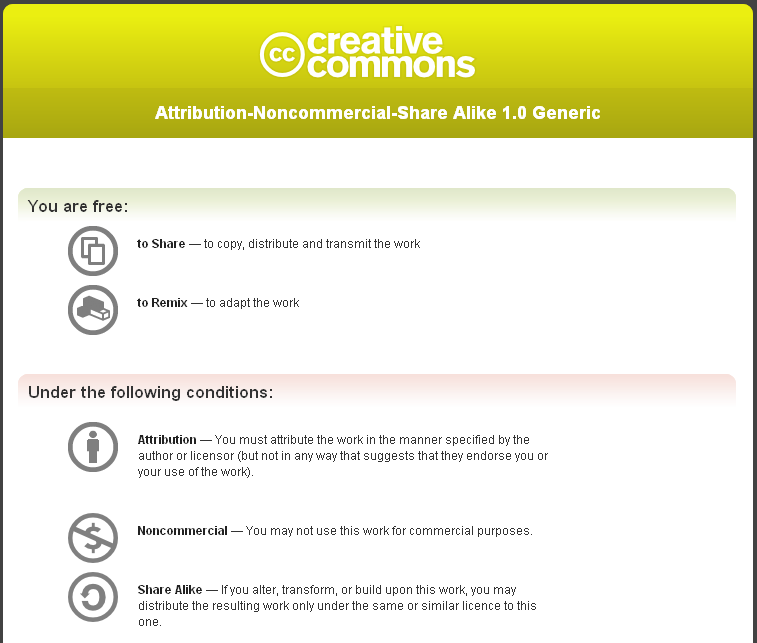
\includegraphics[width=0.50\textwidth]
		{pics/creative_common.png}
	\caption{\license.}
	\label{fig:testGambar}
\end{figure}


%-----------------------------------------------------------------------------%
\section{Membuat Tabel}
%-----------------------------------------------------------------------------%
Seperti pada gambar, tabel juga dapat diberi label dan caption. 
Caption pada tabel terletak pada bagian atas tabel. 
Contoh tabel sederhana dapat dilihat pada \tab~\ref{tab:tab1}.

\begin{table}
	\centering
	\caption{Contoh Tabel}
	\label{tab:tab1}
	\begin{tabular}{| l | c r |}
		\hline
		& kol 1 & kol 2 \\ 
		\hline
		baris 1 & 1 & 2 \\
		baris 2 & 3 & 4 \\
		baris 3 & 5 & 6 \\
		jumlah  & 9 & 12 \\
		\hline
	\end{tabular}
\end{table}

Ada jenis tabel lain yang dapat dibuat dengan \latex~berikut 
beberapa diantaranya. 
Contoh-contoh ini bersumber dari 
\url{http://en.wikibooks.org/wiki/LaTeX/Tables}

\begin{table}
	\centering
	\caption{An Example of Rows Spanning Multiple Columns}
	\label{row.spanning}
	\begin{tabular}{|l|l|*{6}{c|}}
  		\hline % create horizontal line
  		No & Name & \multicolumn{3}{|c|}{Week 1} & \multicolumn{3}{|c|}{Week 2} \\
  		\cline{3-8} % create line from 3rd column till 8th column
  		& & A & B & C & A & B & C\\
  		\hline
  		1 & Lala & 1 & 2 & 3 & 4 & 5 & 6\\
  		2 & Lili & 1 & 2 & 3 & 4 & 5 & 6\\
  		3 & Lulu & 1 & 2 & 3 & 4 & 5 & 6\\
  		\hline
	\end{tabular}
\end{table}

\begin{table}
	\centering
	\caption{An Example of Columns Spanning Multiple Rows}
	\label{column.spanning}
	\begin{tabular}{|l|c|l|}
		\hline
		Percobaan & Iterasi & Waktu \\
		\hline
		Pertama & 1 & 0.1 sec \\ \hline
		\multirow{2}{*}{Kedua} & 1 & 0.1 sec \\
 		& 3 & 0.15 sec \\ 
 		\hline
		\multirow{3}{*}{Ketiga} & 1 & 0.09 sec \\
 		& 2 & 0.16 sec \\
 		& 3 & 0.21 sec \\ 
 		\hline
	\end{tabular}
\end{table}

\begin{table}
	\centering
	\caption{An Example of Spanning in Both Directions Simultaneously}
	\label{mix.spanning}
	\begin{tabular}{cc|c|c|c|c|}
		\cline{3-6}
		& & \multicolumn{4}{|c|}{Title} \\ \cline{3-6}
		& & A & B & C & D \\ \hline
		\multicolumn{1}{|c|}{\multirow{2}{*}{Type}} &
		\multicolumn{1}{|c|}{X} & 1 & 2 & 3 & 4\\ \cline{2-6}
		\multicolumn{1}{|c|}{}                        &
		\multicolumn{1}{|c|}{Y} & 0.5 & 1.0 & 1.5 & 2.0\\ \cline{1-6}
		\multicolumn{1}{|c|}{\multirow{2}{*}{Resource}} &
		\multicolumn{1}{|c|}{I} & 10 & 20 & 30 & 40\\ \cline{2-6}
		\multicolumn{1}{|c|}{}                        &
		\multicolumn{1}{|c|}{J} & 5 & 10 & 15 & 20\\ \cline{1-6}
	\end{tabular}
\end{table}


%-----------------------------------------------------------------------------%
\chapter{\babTiga}
%-----------------------------------------------------------------------------%
\todo{tambahkan kata-kata pengantar bab 1 disini}


%-----------------------------------------------------------------------------%
\section{Satu Persamaan}
%-----------------------------------------------------------------------------%

\noindent \begin{align}\label{eq:garis}
	\cfrac{y - y_{1}}{y_{2} - y_{1}} = 
	\cfrac{x - x_{1}}{x_{2} - x_{1}}
\end{align}

\equ~\ref{eq:garis} diatas adalah persamaan garis. 
\equ~\ref{eq:garis} dan \ref{eq:bola} sama-sama dibuat dengan perintah \bslash
align. 
Perintah ini juga dapat digunakan untuk menulis lebih dari satu persamaan. 

\noindent \begin{align}\label{eq:bola}
	\underbrace{|\overline{ab}|}_{\text{pada bola $|\overline{ab}| = r$}} 
		= \sqrt[2]{(x_{b} - x_{a})^{2} + (y_{b} - y_{a})^{2} + 
				\vert\vert(z_{b} - z_{a})^{2}}
\end{align}

%-----------------------------------------------------------------------------%
\section{Lebih dari Satu Persamaan}
\label{sec:multiEqu}
%-----------------------------------------------------------------------------%
\noindent \begin{align}\label{eq:matriks}	
	|\overline{a} * \overline{b}| &= |\overline{a}| |\overline{b}| \sin\theta 
		\\[0.2cm]
	\overline{a} * \overline{b} &=  
		\begin{array}{| c c c |}
			\hat{i} & x_{1} & x_{2} \\
			\hat{j} & y_{1} & y_{2} \\
			\hat{k} & z_{1} & z_{2} \\
		\end{array} \nonumber \\[0.2cm]
	&= \hat{i} \,
		\begin{array}{ | c c | }
			y_{1} & y_{2} \\
			z_{1} & z_{2} \\
		\end{array} 
	   + \hat{j} \,
		\begin{array}{ | c c | }
			z_{1} & z_{2} \\
			x_{1} & x_{2} \\
		\end{array} 
	   + \hat{k} \,	
		\begin{array}{ | c c | }
			x_{1} & x_{2} \\
			y_{1} & y_{2} \\
		\end{array}
		\nonumber
\end{align}

Pada \equ~\ref{eq:matriks} dapat dilihat beberapa baris menjadi satu bagian 
dari \equ~\ref{eq:matriks}. 
Sedangkan dibawah ini dapat dilihat bahwa dengan cara yang sama, \equ~
\ref{eq:gabungan1}, \ref{eq:gabungan2}, dan \ref{eq:gabungan3} memiliki nomor 
persamaannya masing-masing. 

\noindent \begin{align}\label{eq:gabungan1}	
	\int_{a}^{b} f(x)\, dx + \int_{b}^{c} f(x) \, dx = \int_{a}^{c} f(x) \, dx
		\\\label{eq:gabungan2}
	\lim_{x \to \infty} \frac{f(x)}{g(x)} = 0 \hspace{1cm} 
		\text{jika pangkat $f(x)$ $<$ pangkat $g(x)$} \\\label{eq:gabungan3}
	a^{m^{a \, ^{n}\log b }} = b^{\frac{m}{n}}
\end{align}


%-----------------------------------------------------------------------------%
\chapter{\babEmpat}
%-----------------------------------------------------------------------------%
\todo{tambahkan kata-kata pengantar bab 1 disini}

%-----------------------------------------------------------------------------%
\section{thesis.tex}
%-----------------------------------------------------------------------------%
Berkas ini berisi seluruh berkas Latex yang dibaca, jadi bisa dikatakan sebagai 
berkas utama. Dari berkas ini kita dapat mengatur bab apa saja yang ingin 
kita tampilkan dalam dokumen.


%-----------------------------------------------------------------------------%
\section{laporan\_setting.tex}
%-----------------------------------------------------------------------------%
Berkas ini berguna untuk mempermudah pembuatan beberapa template standar. 
Anda diminta untuk menuliskan judul laporan, nama, npm, dan hal-hal lain yang 
dibutuhkan untuk pembuatan template. 


%-----------------------------------------------------------------------------%
\section{istilah.tex}
%-----------------------------------------------------------------------------%
Berkas istilah digunakan untuk mencatat istilah-istilah yang digunakan. 
Fungsinya hanya untuk memudahkan penulisan.
Pada beberapa kasus, ada kata-kata yang harus selalu muncul dengan tercetak 
miring atau tercetak tebal. 
Dengan menjadikan kata-kata tersebut sebagai sebuah perintah \latex~tentu akan 
mempercepat dan mempermudah pengerjaan laporan. 


%-----------------------------------------------------------------------------%
\section{hype.indonesia.tex}
%-----------------------------------------------------------------------------%
Berkas ini berisi cara pemenggalan beberapa kata dalam bahasa Indonesia. 
\latex~memiliki algoritma untuk memenggal kata-kata sendiri, namun untuk 
beberapa kasus algoritma ini memenggal dengan cara yang salah. 
Untuk memperbaiki pemenggalan yang salah inilah cara pemenggalan yang benar 
ditulis dalam berkas hype.indonesia.tex.


%-----------------------------------------------------------------------------%
\section{pustaka.tex}
%-----------------------------------------------------------------------------%
Berkas pustaka.tex berisi seluruh daftar referensi yang digunakan dalam 
laporan. 
Anda bisa membuat model daftar referensi lain dengan menggunakan bibtex.
Untuk mempelajari bibtex lebih lanjut, silahkan buka 
\url{http://www.bibtex.org/Format}. 
Untuk merujuk pada salah satu referensi yang ada, gunakan perintah \bslash 
cite, e.g. \bslash cite\{latex.intro\} yang akan akan memunculkan 
\cite{latex.intro}


%-----------------------------------------------------------------------------%
\section{bab[1 - 6].tex}
%-----------------------------------------------------------------------------%
Berkas ini berisi isi laporan yang Anda tulis. 
Setiap nama berkas e.g. bab1.tex merepresentasikan bab dimana tulisan tersebut 
akan muncul. 
Sebagai contoh, kode dimana tulisan ini dibaut berada dalam berkas dengan nama 
bab4.tex. 
Ada enam buah berkas yang telah disiapkan untuk mengakomodir enam bab dari 
laporan Anda, diluar bab kesimpulan dan saran. 
Jika Anda tidak membutuhkan sebanyak itu, silahkan hapus kode dalam berkas 
thesis.tex yang memasukan berkas \latex~yang tidak dibutuhkan;  contohnya 
perintah \bslash include\{bab6.tex\} merupakan kode untuk memasukan berkas 
bab6.tex kedalam laporan.


%-----------------------------------------------------------------------------%
\chapter{\babLima}
%-----------------------------------------------------------------------------%

Bab ini menjelaskan hasil pengujian yang dilakukan terhadap perangkat yang dibuat untuk menguji apakah hasil implementasi berjalan sesuai seperti yang diharapkan atau tidak. Penjelasan meliputi perangkat yang digunakan dan hasil pengujian.

\section{Perangkat yang Digunakan}

Perangkat yang digunakan dalam pengujian ini adalah dua buah lampu yang akan dikontrol. Masing-masing lampu ini adalah sebuah lampu berbasis ZigBee dengan merek Philips Hue. Philips Hue adalah sebuah lampu ZigBee yang mengimplementasikan profil ZigBee \textit{Light Link}. Philips Hue merupakan sebuah \textit{Color Dimmable Light}, sehingga dapat diubah warnanya dan tingkat kecerahannya. Gambar \ref{fig:philips-hue} menunujukkan foto kedua lampu yang digunakan.

\begin{figure}
	\centering
	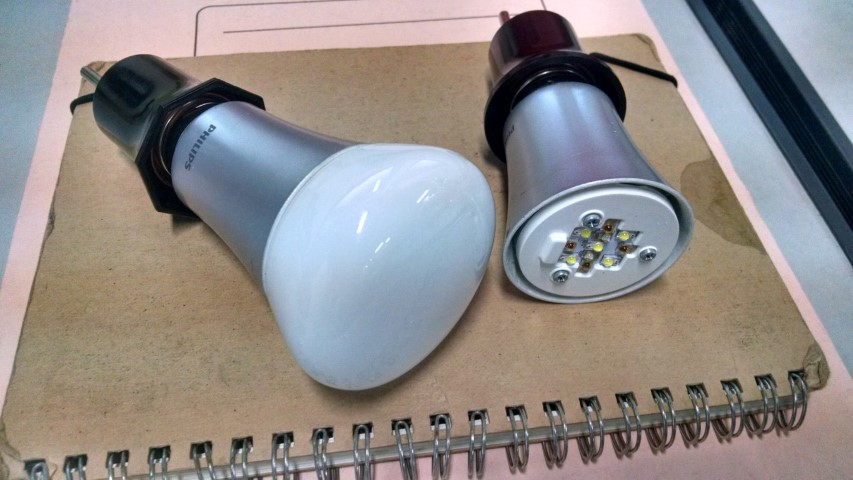
\includegraphics[width=.9\textwidth]{pics/philips-hue.jpg}
	\caption{Lampu Philips Hue yang digunakan untuk pengujian}
	\label{fig:philips-hue}
\end{figure}

\subsection{Hasil Pengujian}
\begin{enumerate}
	\item Kasus Uji 1: Menjadi \textit{access point}.
	\begin{table}
		\centering
		\caption{Hasil pengujian kasus uji 1}
		\label{tab:kasusUji1}
		\begin{tabular}{| l | p{11cm} |}
			\hline
			\textbf{Perintah} & Perangkat \textit{gateway} dinyalakan \\
			\hline
			\textbf{Prekondisi} & -\\
			\hline
			\textbf{Hasil} & Perangkat \textit{gateway} menyala dengan \textit{access point} bernama "ZigBee\_Gateway" muncul
			
			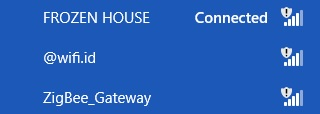
\includegraphics[width=.75\textwidth]{pics/uji1.jpg}\\
			\hline
			\textbf{Ekspektasi} & \textit{Access point} bernama "ZigBee\_Gateway" muncul \\
			\hline
		\end{tabular}
	\end{table}
		\item Kasus Uji 2: Menghubungkan perangkat \textit{gateway} ke \textit{access point} lain.
		\begin{table}
			\centering
			\caption{Hasil pengujian kasus uji 2}
			\label{tab:kasusUji2}
			\begin{tabular}{| l | p{11cm} |}
				\hline
				\textbf{Perintah} & Membuka halaman \code{192.168.42.1/ta/wifi.php}, dan memilih salah satu \textit{access point} lain \\
				\hline
				\textbf{Prekondisi} & Perangkat yang digunakan untuk mengakses sudah terhubung ke perangkat \textit{gateway}\\
				\hline
				\textbf{Hasil} & Perangkat \textit{gateway} terhubung ke \textit{access point} yang dipilih dan mendapatkan alamat IP \code{192.168.1.135}.
				
				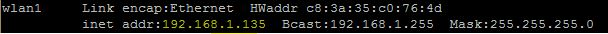
\includegraphics[width=.75\textwidth]{pics/uji1x.jpg}\\
				\hline
				\textbf{Ekspektasi} & Perangkat \textit{gateway} terhubung ke \textit{access point} yang dipilih dan mendapatkan sebuah alamat IP \\
				\hline
			\end{tabular}
		\end{table}
	\item Kasus Uji 3: Menyalakan lampu melalui halaman web pada perangkat \textit{gateway}
	\begin{table}
		\centering
		\caption{Hasil pengujian kasus uji 3}
		\label{tab:kasusUji3}
		\begin{tabular}{| l | p{11cm} |}
			\hline
			\textbf{Perintah} & Tombol 'Nyalakan' ditekan \\
			\hline
			\textbf{Prekondisi} & Perangkat \textit{gateway} sudah berjalan, lampu sudah terhubung dengan perangkat \textit{gateway} dan dalam keadaan mati\\
			\hline
			\textbf{Hasil} & Lampu menyala 
			
			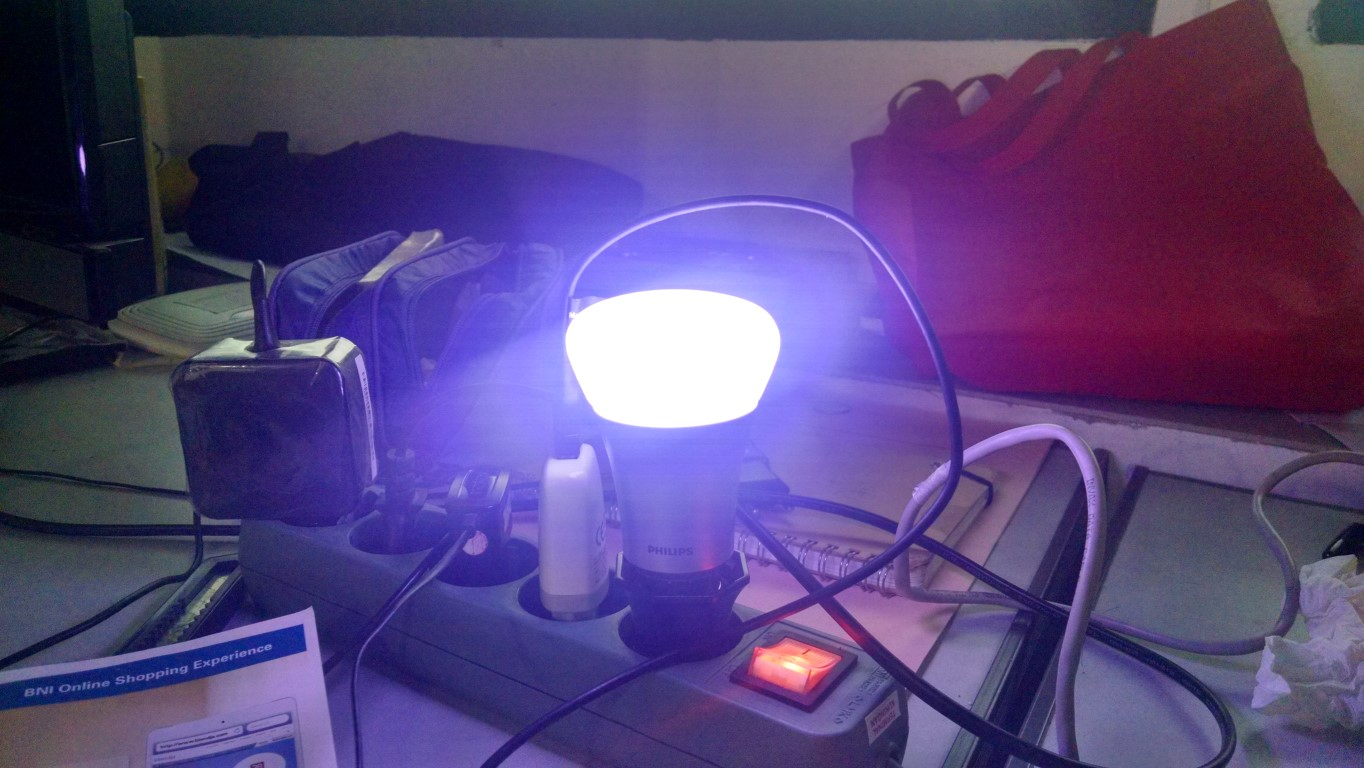
\includegraphics[width=.75\textwidth]{pics/uji2.jpg}\\
			\hline
			\textbf{Ekspektasi} & Lampu menyala \\
			\hline
		\end{tabular}
	\end{table}
	\item Kasus Uji 4: Mematikan lampu melalui halaman web pada perangkat \textit{gateway}
	\begin{table}
		\centering
		\caption{Hasil pengujian kasus uji 4}
		\label{tab:kasusUji4}
		\begin{tabular}{| l | p{11cm} |}
			\hline
			\textbf{Perintah} & Tombol 'Matikan' ditekan \\
			\hline
			\textbf{Prekondisi} & Perangkat \textit{gateway} sudah berjalan, lampu sudah terhubung dengan perangkat  \textit{gateway} dan dalam keadaan menyala\\
			\hline
			\textbf{Hasil} & Lampu mati 
			
			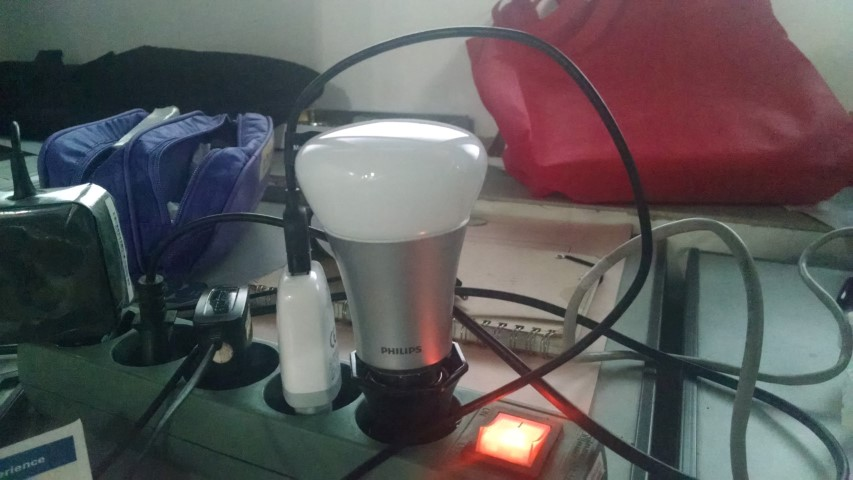
\includegraphics[width=.75\textwidth]{pics/uji3.jpg}\\
			\hline
			\textbf{Ekspektasi} & Lampu mati \\
			\hline
		\end{tabular}
	\end{table}
	\item Kasus Uji 5: Mengubah tingkat kecerahan lampu melalui halaman web pada perangkat \textit{gateway}
	\begin{table}
		\centering
		\caption{Hasil pengujian kasus uji 5}
		\label{tab:kasusUji5}
		\begin{tabular}{| l | p{11cm} |}
			\hline
			\textbf{Perintah} & \textit{Slider} tingkat kecerahan digeser ke nilai yang lebih tinggi \\
			\hline
			\textbf{Prekondisi} & Perangkat \textit{gateway} sudah berjalan, lampu sudah terhubung dengan perangkat  \textit{gateway} dan dalam keadaan menyala\\
			\hline
			\textbf{Hasil} & Lampu menjadi lebih terang 
			
			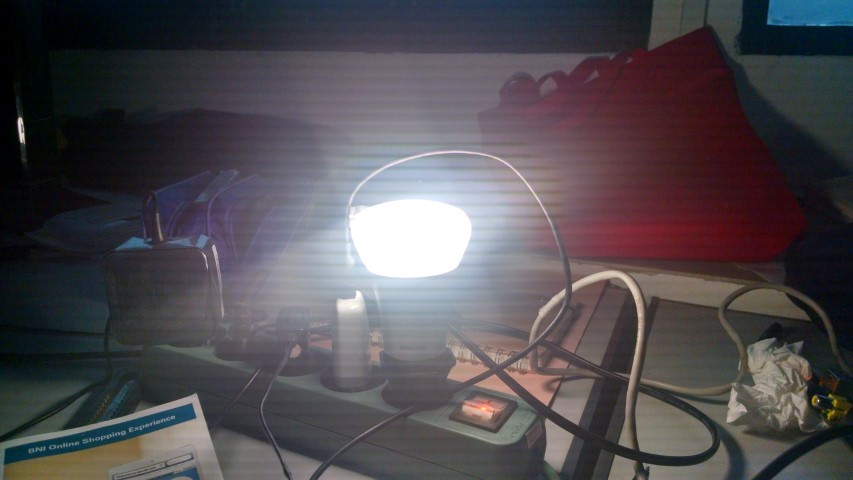
\includegraphics[width=.75\textwidth]{pics/uji4.jpg}\\
			\hline
			\textbf{Ekspektasi} & Lampu menjadi lebih terang \\
			\hline
		\end{tabular}
	\end{table}
	\item Kasus Uji 6: Mengubah warna lampu melalui halaman web pada perangkat \textit{gateway}
	\begin{table}
		\centering
		\caption{Hasil pengujian kasus uji 6}
		\label{tab:kasusUji6}
		\begin{tabular}{| l | p{11cm} |}
			\hline
			\textbf{Perintah} & Mengubah warna pada \textit{color picker} menjadi berwarna merah \\
			\hline
			\textbf{Prekondisi} & Perangkat \textit{gateway} sudah berjalan, lampu sudah terhubung dengan perangkat  \textit{gateway} dan dalam keadaan menyala\\
			\hline
			\textbf{Hasil} & Lampu menjadi berwarna merah 
			
			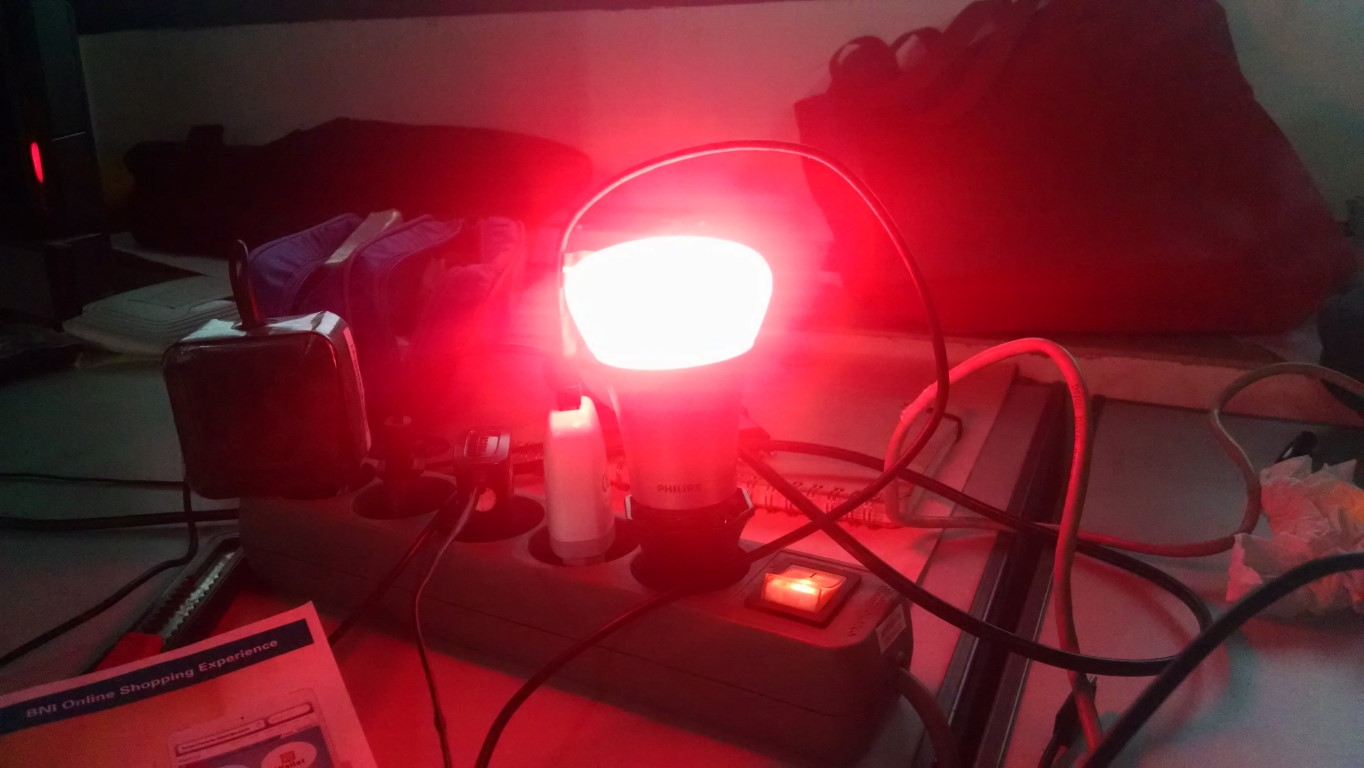
\includegraphics[width=.75\textwidth]{pics/uji5.jpg}\\
			\hline
			\textbf{Ekspektasi} & Lampu menjadi berwarna merah \\
			\hline
		\end{tabular}
	\end{table}
	\item Kasus Uji 7: Mengubah tingkat kejenuhan lampu melalui halaman web pada perangkat \textit{gateway}
	\begin{table}
		\centering
		\caption{Hasil pengujian kasus uji 7}
		\label{tab:kasusUji7}
		\begin{tabular}{| l | p{11cm} |}
			\hline
			\textbf{Perintah} & Menurunkan tingkat kejenuhan warna menggunakan \textit{color picker} \\
			\hline
			\textbf{Prekondisi} & Perangkat \textit{gateway} sudah berjalan, lampu sudah terhubung dengan perangkat  \textit{gateway} dan dalam keadaan menyala\\
			\hline
			\textbf{Hasil} & Lampu menjadi berwarna lebih muda 
			
			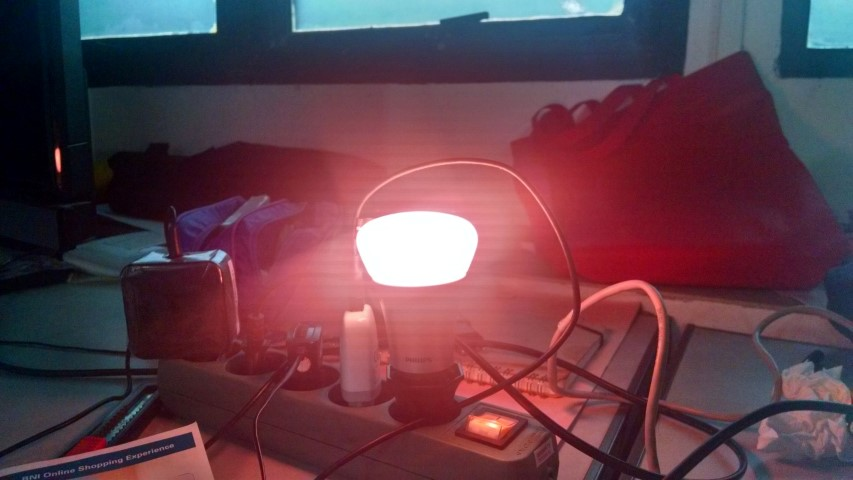
\includegraphics[width=.75\textwidth]{pics/uji6.jpg}\\
			\hline
			\textbf{Ekspektasi} & Lampu menjadi berwarna lebih muda \\
			\hline
		\end{tabular}
	\end{table}
	\item Kasus Uji 8: Membuat sebuah \textit{group} melalui halaman web pada perangkat \textit{gateway}
	\begin{table}
		\centering
		\caption{Hasil pengujian kasus uji 8}
		\label{tab:kasusUji8}
		\begin{tabular}{| l | p{11cm} |}
			\hline
			\textbf{Perintah} & Menekan tombol 'Buat Group', mengisi nama, kemudian memilih 'Light 1' dan 'Light 2', dan menekan tombol 'submit' \\
			\hline
			\textbf{Prekondisi} & Perangkat \textit{gateway} sudah berjalan, lampu sudah terhubung dengan perangkat \textit{gateway}\\
			\hline
			\textbf{Hasil} & Group terdaftar dengan anggota 'Light 1' dan 'Light 2'\\
			\hline
			\textbf{Ekspektasi} & Group terdaftar dengan anggota 'Light 1' dan 'Light 2' \\
			\hline
		\end{tabular}
	\end{table}
	\item Kasus Uji 9: Menyalakan lampu dalam suatu \textit{group} melalui halaman web pada perangkat \textit{gateway}
	\begin{table}
		\centering
		\caption{Hasil pengujian kasus uji 9}
		\label{tab:kasusUji9}
		\begin{tabular}{| l | p{11cm} |}
			\hline
			\textbf{Perintah} & Tombol 'Nyalakan' pada bagian \textit{groups} ditekan \\
			\hline
			\textbf{Prekondisi} & Perangkat \textit{gateway} sudah berjalan, lampu sudah terhubung dengan perangkat \textit{gateway}, \textit{group} sudah dibuat, dan lampu dalam keadaan mati \\
			\hline
			\textbf{Hasil} & Kedua lampu menyala 
			
			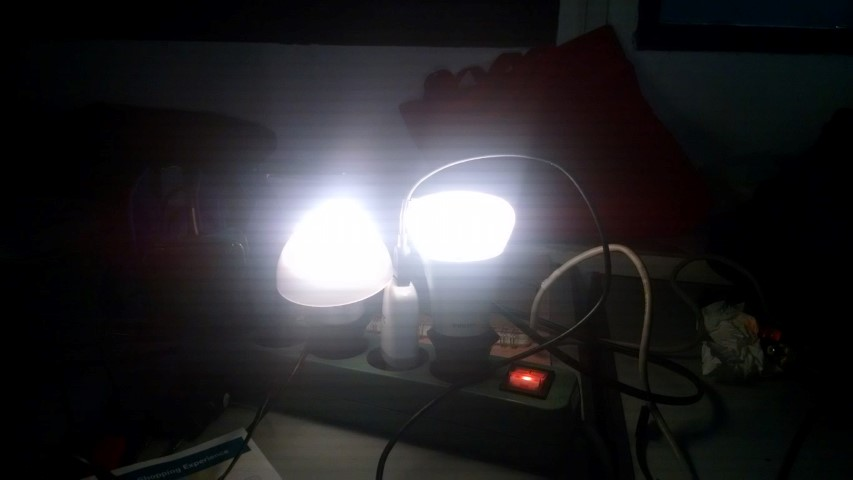
\includegraphics[width=.75\textwidth]{pics/uji8.jpg}\\
			\hline
			\textbf{Ekspektasi} & Kedua lampu menyala \\
			\hline
		\end{tabular}
	\end{table}
	\item Kasus Uji 10: Mematikan lampu dalam suatu \textit{group} melalui halaman web pada perangkat \textit{gateway}
	\begin{table}
		\centering
		\caption{Hasil pengujian kasus uji 10}
		\label{tab:kasusUji10}
		\begin{tabular}{| l | p{11cm} |}
			\hline
			\textbf{Perintah} & Tombol 'Matikan' pada bagian \textit{groups} ditekan \\
			\hline
			\textbf{Prekondisi} & Perangkat \textit{gateway} sudah berjalan, lampu sudah terhubung dengan perangkat \textit{gateway}, \textit{group} sudah dibuat, dan lampu dalam keadaan menyala \\
			\hline
			\textbf{Hasil} & Kedua lampu mati 
			
			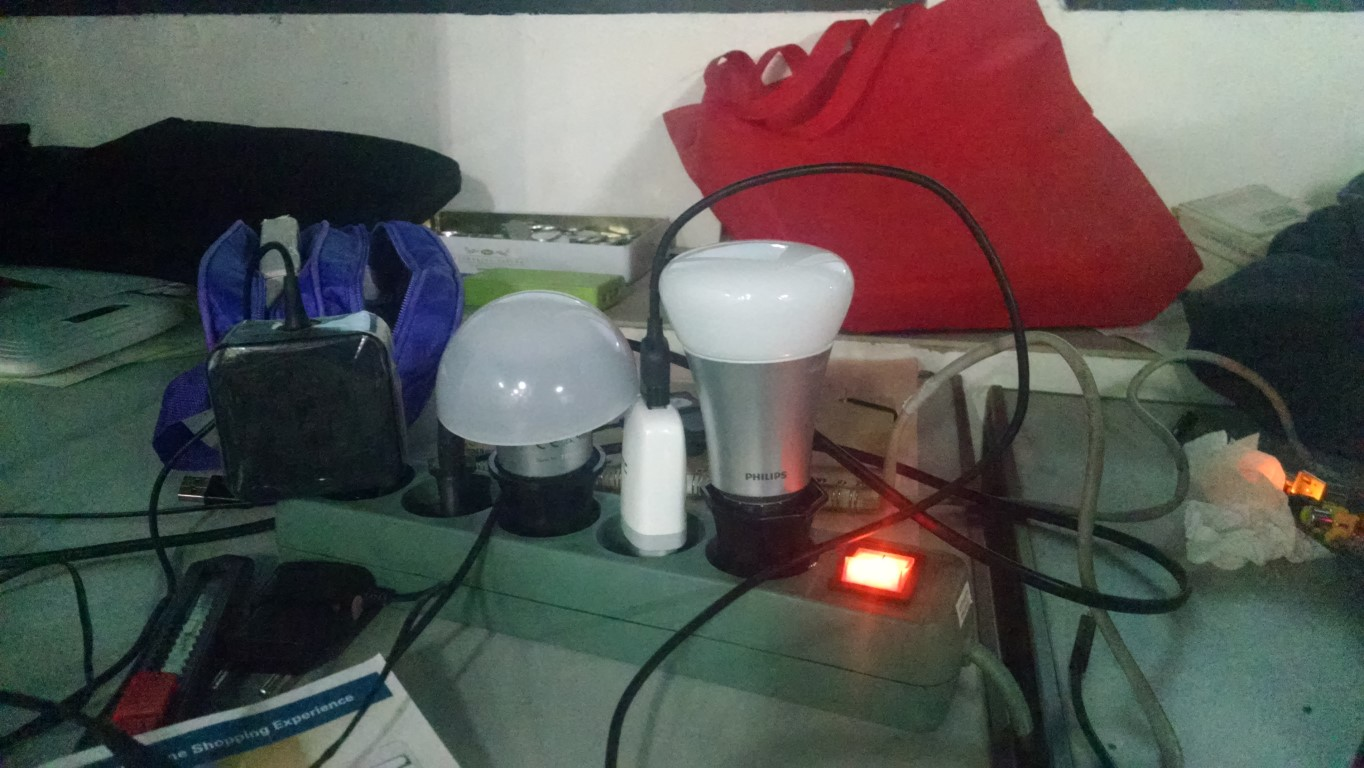
\includegraphics[width=.75\textwidth]{pics/uji9.jpg}\\
			\hline
			\textbf{Ekspektasi} & Kedua lampu mati \\
			\hline
		\end{tabular}
	\end{table}
	\item Kasus Uji 11: Mengubah tingkat kecerahan lampu dalam suatu \textit{group} melalui halaman web pada perangkat \textit{gateway}
	\begin{table}
		\centering
		\caption{Hasil pengujian kasus uji 11}
		\label{tab:kasusUji11}
		\begin{tabular}{| l | p{11cm} |}
			\hline
			\textbf{Perintah} & \textit{Slider} tingkat kecerahan pada bagian \textit{groups} digeser ke nilai yang lebih tinggi\\
			\hline
			\textbf{Prekondisi} & Perangkat \textit{gateway} sudah berjalan, lampu sudah terhubung dengan perangkat \textit{gateway}, \textit{group} sudah dibuat, dan lampu dalam keadaan menyala \\
			\hline
			\textbf{Hasil} & Kedua lampu menjadi lebih terang 
			
			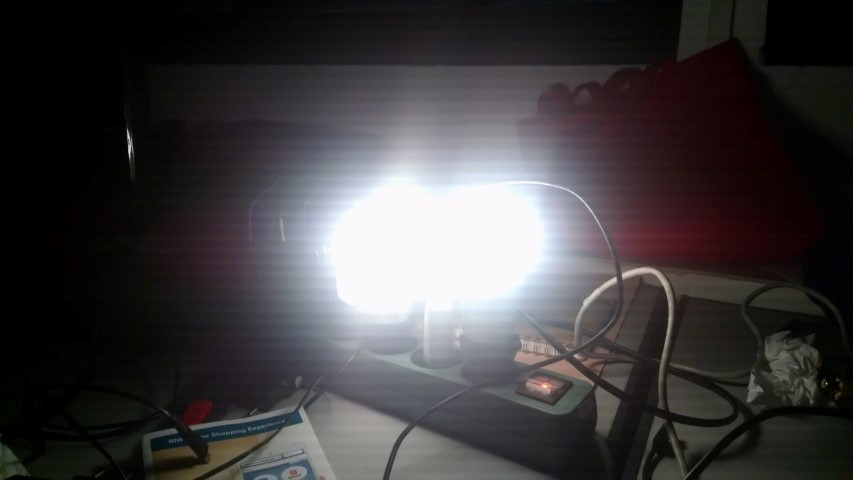
\includegraphics[width=.75\textwidth]{pics/uji10.jpg}\\
			\hline
			\textbf{Ekspektasi} & Kedua lampu menjadi lebih terang \\
			\hline
		\end{tabular}
	\end{table}
	\item Kasus Uji 12: Mengubah warna lampu dalam suatu \textit{group} melalui halaman web pada perangkat \textit{gateway}
	\begin{table}
		\centering
		\caption{Hasil pengujian kasus uji 12}
		\label{tab:kasusUji12}
		\begin{tabular}{| l | p{11cm} |}
			\hline
			\textbf{Perintah} & Mengubah warna pada \textit{color picker} menjadi berwarna hijau\\
			\hline
			\textbf{Prekondisi} & Perangkat \textit{gateway} sudah berjalan, lampu sudah terhubung dengan perangkat \textit{gateway}, \textit{group} sudah dibuat, dan lampu dalam keadaan menyala \\
			\hline
			\textbf{Hasil} & Kedua lampu menjadi berwarna hijau 
			
			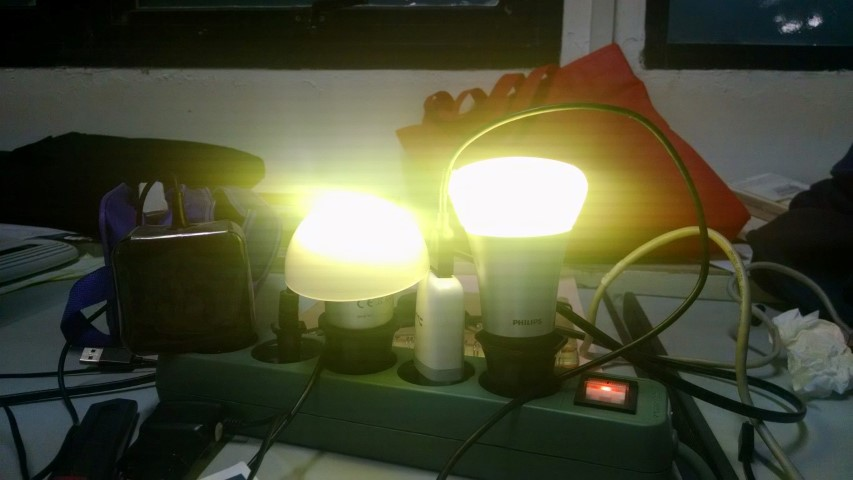
\includegraphics[width=.75\textwidth]{pics/uji11.jpg}\\
			\hline
			\textbf{Ekspektasi} & Kedua lampu menjadi berwarna hijau \\
			\hline
		\end{tabular}
	\end{table}
	\item Kasus Uji 13: Mengubah tingkat kejenuhan lampu dalam suatu \textit{group} melalui halaman web pada perangkat \textit{gateway}
	\begin{table}
		\centering
		\caption{Hasil pengujian kasus uji 13}
		\label{tab:kasusUji13}
		\begin{tabular}{| l | p{11cm} |}
			\hline
			\textbf{Perintah} & Mengubah tingkat kejenuhan warna menggunakan \textit{color picker} pada bagian \textit{groups}\\
			\hline
			\textbf{Prekondisi} & Perangkat \textit{gateway} sudah berjalan, lampu sudah terhubung dengan perangkat \textit{gateway}, \textit{group} sudah dibuat, dan lampu dalam keadaan menyala \\
			\hline
			\textbf{Hasil} & Kedua lampu menjadi berwarna berwarna lebih muda 
			
			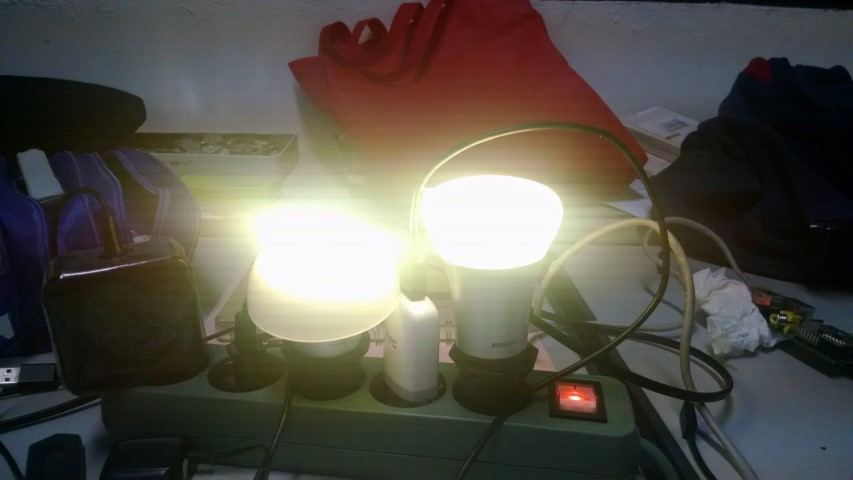
\includegraphics[width=.75\textwidth]{pics/uji12.jpg}\\
			\hline
			\textbf{Ekspektasi} & Kedua lampu menjadi berwarna berwarna lebih muda \\
			\hline
		\end{tabular}
	\end{table}
	\item Kasus Uji 14: Mendaftarkan lampu ke \plat~melalui halaman web pada perangkat \textit{gateway}.
	\begin{table}
		\centering
		\caption{Hasil pengujian kasus uji 14}
		\label{tab:kasusUji14}
		\begin{tabular}{| l | p{11cm} |}
			\hline
			\textbf{Perintah} & Menekan tombol 'Daftarkan Light2', memilih hak akses untuk setiap atribut, dan menekan tombol 'Daftar' \\
			\hline
			\textbf{Prekondisi} & Perangkat \textit{gateway} sudah terhubung ke \textit{access point} dengan koneksi internet, lampu sudah terhubung dengan perangkat \textit{gateway}\\
			\hline
			\textbf{Hasil} & Lampu beserta atribut yang dipilih terdaftar dan mendapat id \code{557d23cb0fcf33af4e209d93}\\
			\hline
			\textbf{Ekspektasi} & Lampu beserta atribut yang dipilih terdaftar dan mendapat sebuah id \\
			\hline
		\end{tabular}
	\end{table}
	\item Kasus Uji 15: Mendaftarkan \textit{group} ke \plat~melalui halaman web pada perangkat \textit{gateway}
	\begin{table}
		\centering
		\caption{Hasil pengujian kasus uji 15}
		\label{tab:kasusUji15}
		\begin{tabular}{| l | p{11cm} |}
			\hline
			\textbf{Perintah} & Menekan tombol 'Daftarkan Lab Nok', memilih hak akses untuk setiap atribut, dan menekan tombol 'Daftar' \\
			\hline
			\textbf{Prekondisi} & Perangkat \textit{gateway} sudah terhubung ke \textit{access point} dengan koneksi internet, \textit{group} sudah dibuat\\
			\hline
			\textbf{Hasil} & \textit{Group} beserta atribut yang dipilih terdaftar dan mendapat id \code{557d10c80fcf33af4e209d8e}\\
			\hline
			\textbf{Ekspektasi} & \textit{Group} beserta atribut yang dipilih terdaftar dan mendapat sebuah id \\
			\hline
		\end{tabular}
	\end{table}
	\item Kasus Uji 16: Mengirimkan informasi mengenai atribut yang didaftarkan secara berkala ke \textit{pub-sub system}
	\begin{table}
		\centering
		\caption{Hasil pengujian kasus uji 16}
		\label{tab:kasusUji16}
		\begin{tabular}{| l | p{11cm} |}
			\hline
			\textbf{Perintah} & \code{mosquitto\_sub -h 128.199.236.53 -t sot/g/557903af5ad821942ef0af51/+/+/+/acc} \\
			\hline
			\textbf{Prekondisi} & Perangkat \textit{gateway} sudah terhubung ke \textit{access point} dengan koneksi internet, lampu sudah terhubung ke perangkat \textit{gateway}\\
			\hline
			\textbf{Hasil} & Mendapatkan informasi mengenai atribut yang didaftarkan setiap sepuluh detik
			
			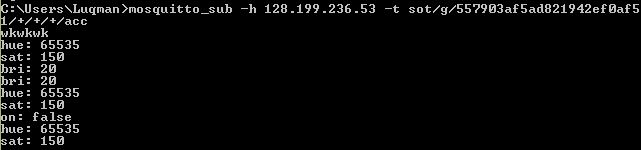
\includegraphics[width=.75\textwidth]{pics/uji15.jpg}\\
			\hline
			\textbf{Ekspektasi} & Mendapatkan informasi mengenai atribut yang didaftarkan setiap sepuluh detik \\
			\hline
		\end{tabular}
	\end{table}
	\item Kasus Uji 17: Menyalakan lampu melalui pesan yang dikirimkan dari \textit{pub-sub system}.
	\begin{table}
		\centering
		\caption{Hasil pengujian kasus uji 17}
		\label{tab:kasusUji17}
		\begin{tabular}{| l | p{11cm} |}
			\hline
			\textbf{Topik} & \code{sot/g/557903af5ad821942ef0af51/ledlight /557b693c1463cee933d9df01/on/ctl}\\
			\hline
			\textbf{Prekondisi} & Lampu sudah didaftarkan dengan atribut terkait diberikan hak kontrol, lampu dalam keadaan mati\\
			\hline
			\textbf{Isi pesan} & \code{true}\\
			\hline
			\textbf{Hasil} & Lampu menyala 
			
			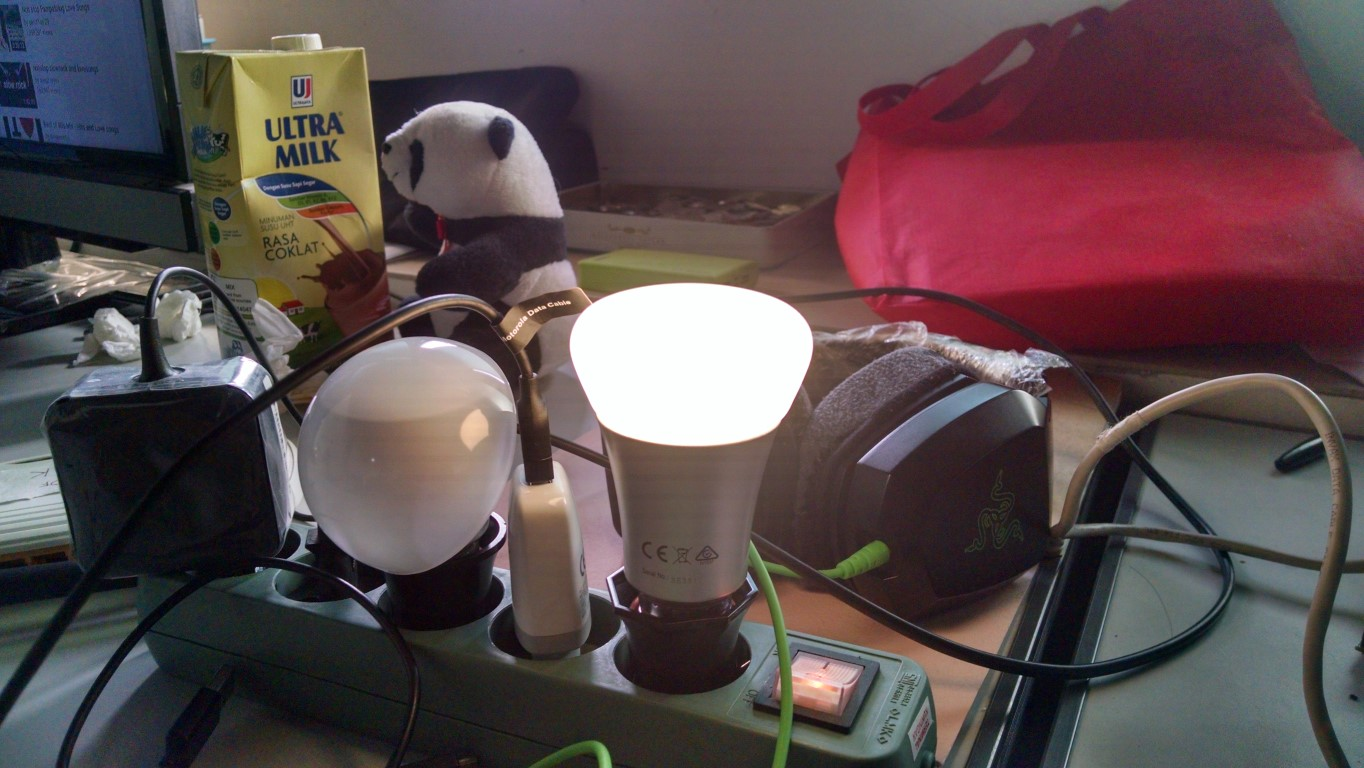
\includegraphics[width=.75\textwidth]{pics/uji16.jpg}\\
			\hline
			\textbf{Ekspektasi} & Lampu menyala \\
			\hline
		\end{tabular}
	\end{table}
	\item Kasus Uji 18: Mematikan lampu melalui pesan yang dikirimkan dari \textit{pub-sub system}.
	\begin{table}
		\centering
		\caption{Hasil pengujian kasus uji 18}
		\label{tab:kasusUji18}
		\begin{tabular}{| l | p{11cm} |}
			\hline
			\textbf{Topik} & \code{sot/g/557903af5ad821942ef0af51/ledlight /557b693c1463cee933d9df01/on/ctl}\\
			\hline
			\textbf{Prekondisi} & Lampu sudah didaftarkan dengan atribut terkait diberikan hak kontrol, lampu dalam keadaan menyala\\
			\hline
			\textbf{Isi pesan} & \code{false}\\
			\hline
			\textbf{Hasil} & Lampu mati 
			
			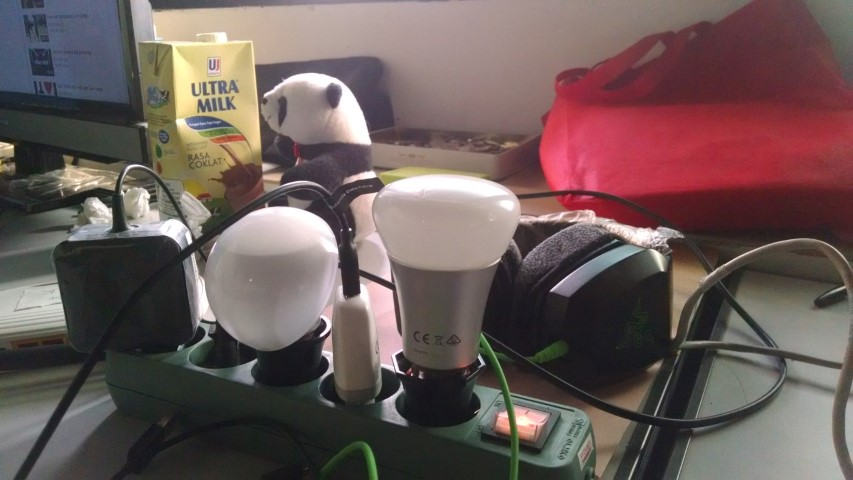
\includegraphics[width=.75\textwidth]{pics/uji17.jpg}\\
			\hline
			\textbf{Ekspektasi} & Lampu mati \\
			\hline
		\end{tabular}
	\end{table}
	\item Kasus Uji 19: Mengubah tingkat kecerahan lampu melalui pesan yang dikirimkan dari \textit{pub-sub system}.
	\begin{table}
		\centering
		\caption{Hasil pengujian kasus uji 19}
		\label{tab:kasusUji19}
		\begin{tabular}{| l | p{11cm} |}
			\hline
			\textbf{Topik} & \code{sot/g/557903af5ad821942ef0af51/ledlight /557b693c1463cee933d9df01/bri/ctl}\\
			\hline
			\textbf{Prekondisi} & Lampu sudah didaftarkan dengan atribut terkait diberikan hak kontrol, lampu dalam keadaan menyala\\
			\hline
			\textbf{Isi pesan} & \code{200}\\
			\hline
			\textbf{Hasil} & Lampu menjadi lebih terang 
			
			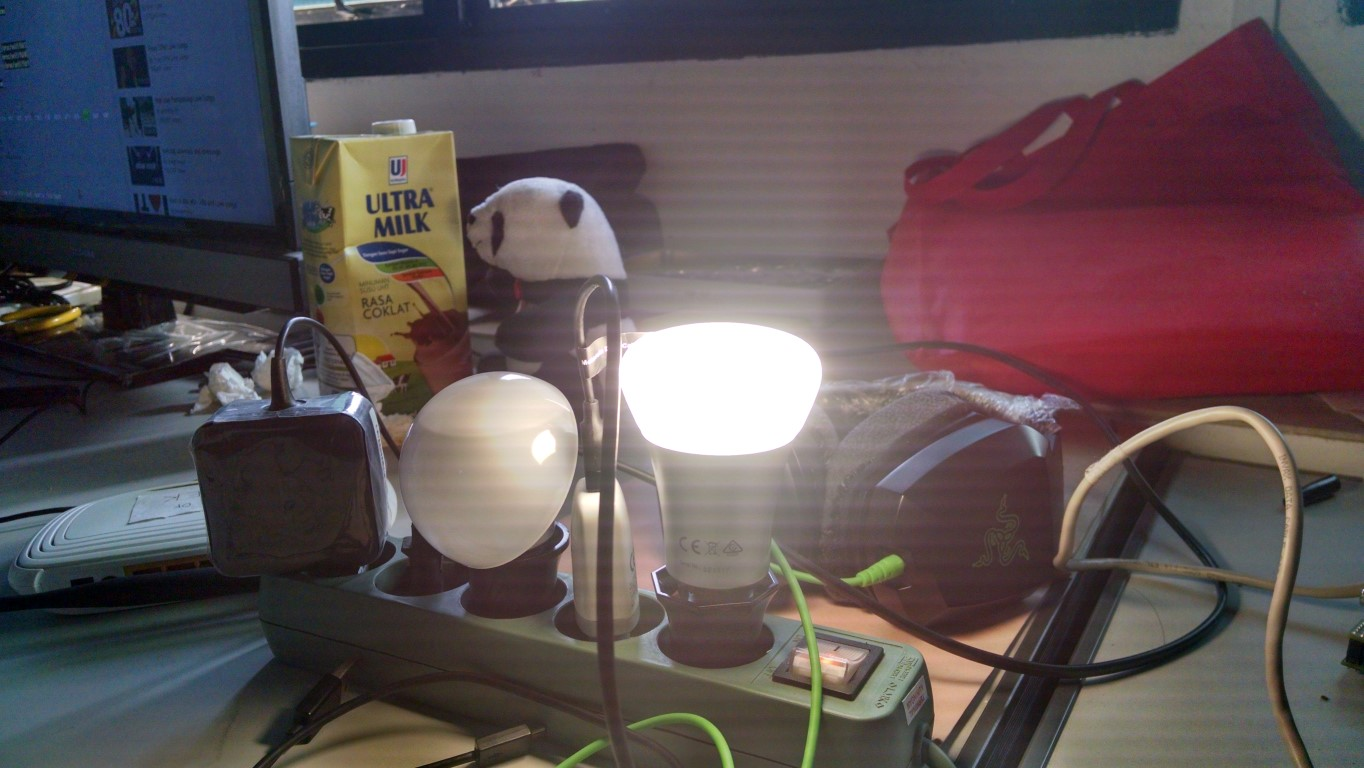
\includegraphics[width=.75\textwidth]{pics/uji18.jpg}\\
			\hline
			\textbf{Ekspektasi} & Lampu menjadi lebih terang  \\
			\hline
		\end{tabular}
	\end{table}
	\item Kasus Uji 20: Mengubah warna lampu melalui pesan yang dikirimkan dari \textit{pub-sub system}.
	\begin{table}
		\centering
		\caption{Hasil pengujian kasus uji 20}
		\label{tab:kasusUji20}
		\begin{tabular}{| l | p{11cm} |}
			\hline
			\textbf{Topik} & \code{sot/g/557903af5ad821942ef0af51/ledlight /557b693c1463cee933d9df01/hue/ctl}\\
			\hline
			\textbf{Prekondisi} & Lampu sudah didaftarkan dengan atribut terkait diberikan hak kontrol, lampu dalam keadaan menyala\\
			\hline
			\textbf{Isi pesan} & \code{45000}\\
			\hline
			\textbf{Hasil} & Lampu menjadi berwarna biru
			
			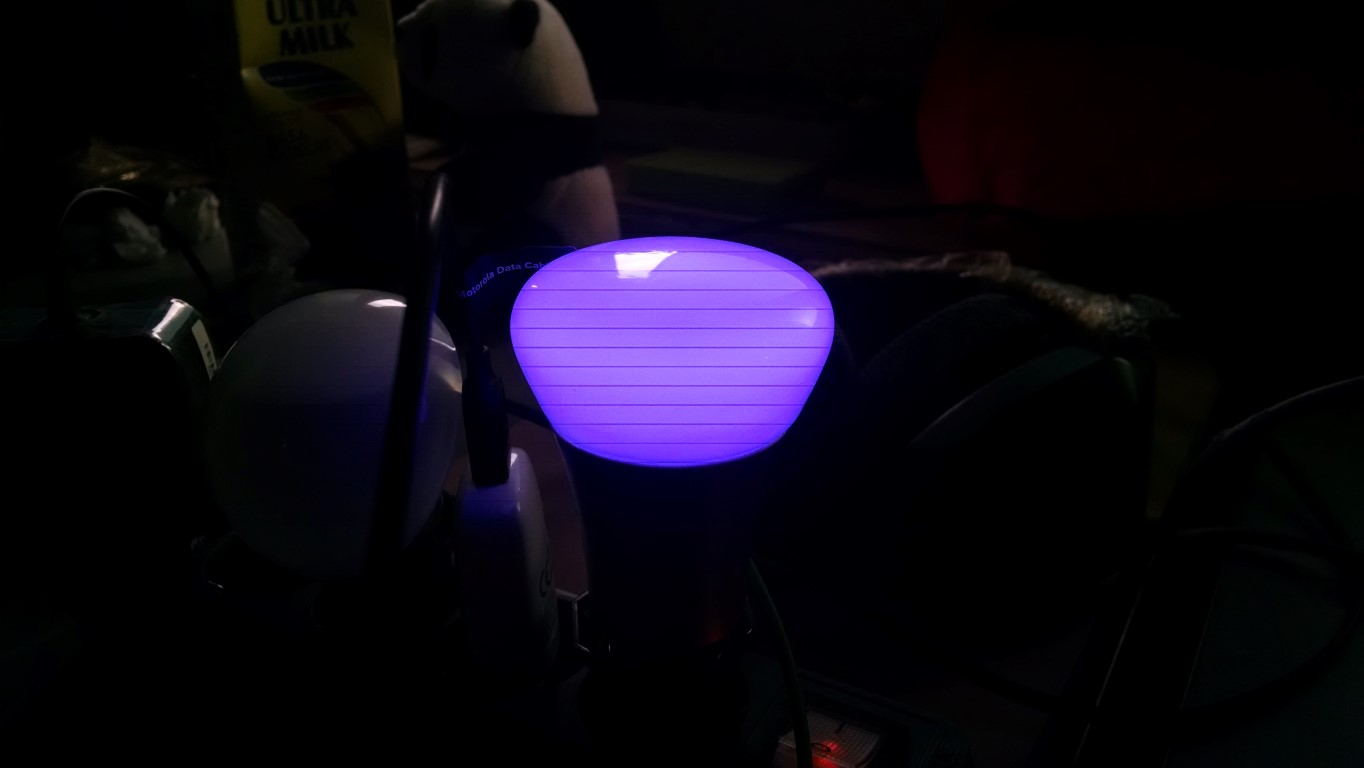
\includegraphics[width=.75\textwidth]{pics/uji19.jpg}\\
			\hline
			\textbf{Ekspektasi} & Lampu menjadi berwarna biru  \\
			\hline
		\end{tabular}
	\end{table}
	\item Kasus Uji 21: Mengubah tingkat kejenuhan lampu melalui pesan yang dikirimkan dari \textit{pub-sub system}.
	\begin{table}
		\centering
		\caption{Hasil pengujian kasus uji 21}
		\label{tab:kasusUji21}
		\begin{tabular}{| l | p{11cm} |}
			\hline
			\textbf{Topik} & \code{sot/g/557903af5ad821942ef0af51/ledlight /557b693c1463cee933d9df01/sat/ctl}\\
			\hline
			\textbf{Prekondisi} & Lampu sudah didaftarkan dengan atribut terkait diberikan hak kontrol, lampu dalam keadaan menyala\\
			\hline
			\textbf{Isi pesan} & \code{150}\\
			\hline
			\textbf{Hasil} & Lampu menjadi berwarna lebih muda
			
			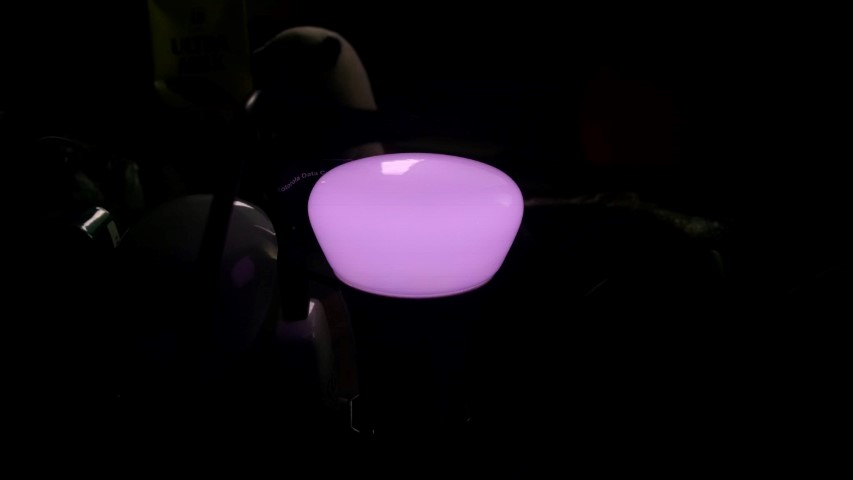
\includegraphics[width=.75\textwidth]{pics/uji20.jpg}\\
			\hline
			\textbf{Ekspektasi} & Lampu menjadi berwarna lebih muda  \\
			\hline
		\end{tabular}
	\end{table}
	\item Kasus Uji 22: Menyalakan lampu dalam suatu \textit{group} melalui pesan yang dikirimkan dari \textit{pub-sub system}.
	\begin{table}
		\centering
		\caption{Hasil pengujian kasus uji 22}
		\label{tab:kasusUji22}
		\begin{tabular}{| l | p{11cm} |}
			\hline
			\textbf{Topik} & \code{sot/g/557903af5ad821942ef0af51/ledlight /557d10c80fcf33af4e209d8e/on/ctl}\\
			\hline
			\textbf{Prekondisi} & \textit{Group} sudah didaftarkan dengan atribut terkait diberikan hak kontrol, lampu anggota \textit{group} dalam keadaan mati\\
			\hline
			\textbf{Isi pesan} & \code{true}\\
			\hline
			\textbf{Hasil} & Kedua lampu menyala 
			
			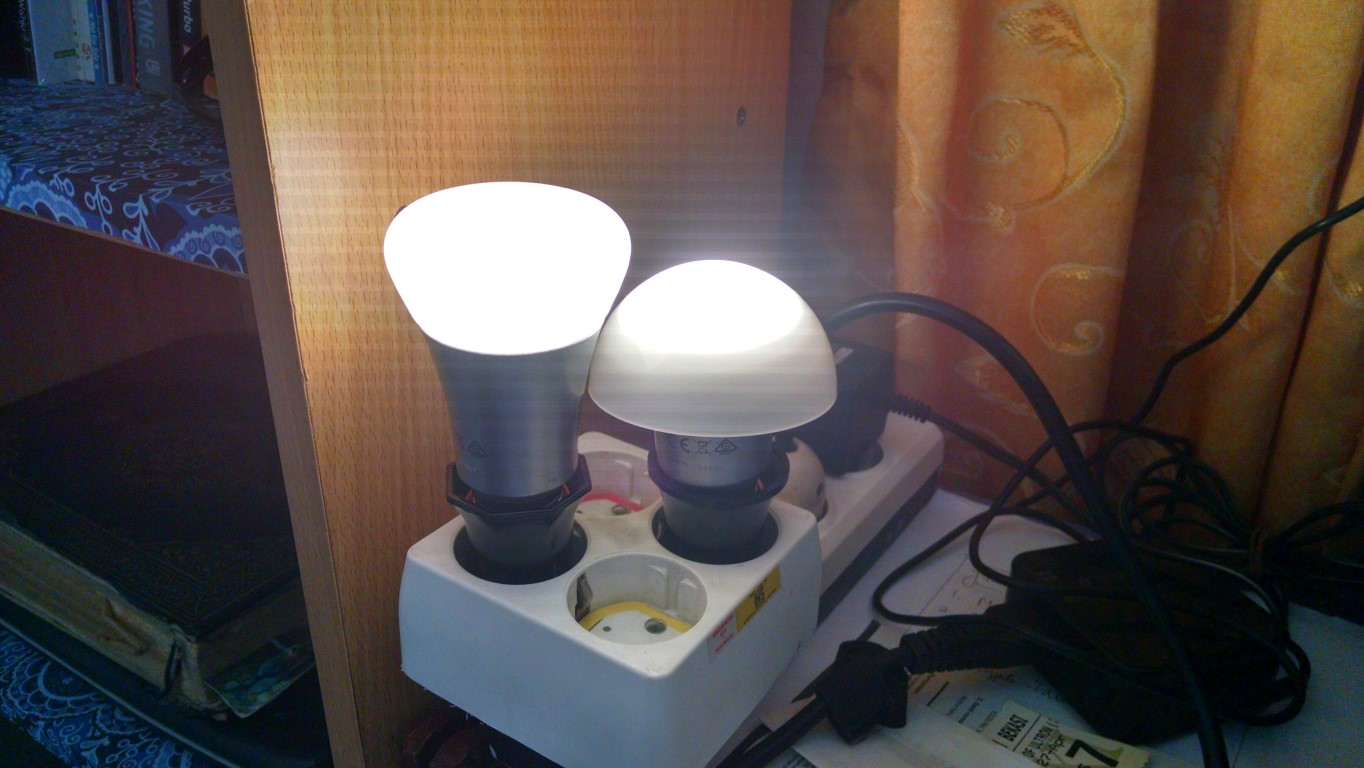
\includegraphics[width=.75\textwidth]{pics/uji21.jpg}\\
			\hline
			\textbf{Ekspektasi} & Kedua lampu menyala  \\
			\hline
		\end{tabular}
	\end{table}
	\item Kasus Uji 23: Mematikan lampu dalam suatu \textit{group} melalui pesan yang dikirimkan dari \textit{pub-sub system}.
	\begin{table}
		\centering
		\caption{Hasil pengujian kasus uji 23}
		\label{tab:kasusUji23}
		\begin{tabular}{| l | p{11cm} |}
			\hline
			\textbf{Topik} & \code{sot/g/557903af5ad821942ef0af51/ledlight /557d10c80fcf33af4e209d8e/on/ctl}\\
			\hline
			\textbf{Prekondisi} & \textit{Group} sudah didaftarkan dengan atribut terkait diberikan hak kontrol, lampu anggota \textit{group} dalam keadaan menyala\\
			\hline
			\textbf{Isi pesan} & \code{false}\\
			\hline
			\textbf{Hasil} & Kedua lampu mati 
			
			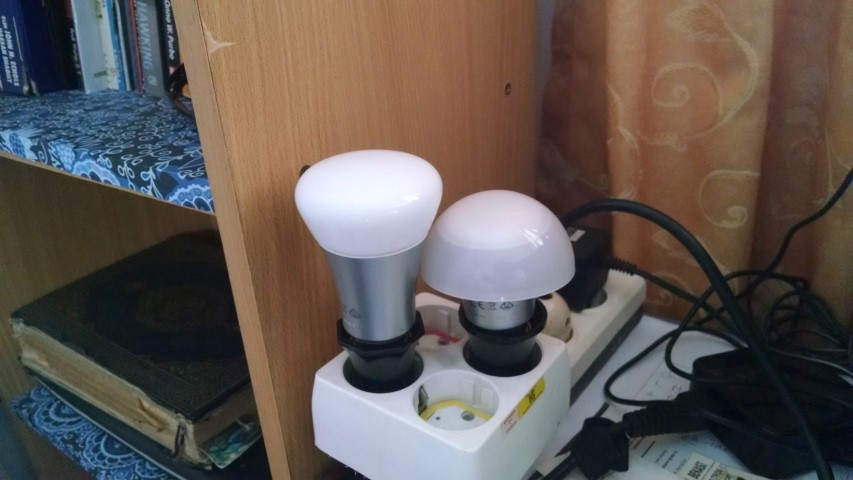
\includegraphics[width=.75\textwidth]{pics/uji22.jpg}\\
			\hline
			\textbf{Ekspektasi} & Kedua lampu mati  \\
			\hline
		\end{tabular}
	\end{table}
	\item Kasus Uji 24: Mengubah tingkat kecerahan lampu dalam suatu \textit{group} melalui pesan yang dikirimkan dari \textit{pub-sub system}.
	\begin{table}
		\centering
		\caption{Hasil pengujian kasus uji 24}
		\label{tab:kasusUji24}
		\begin{tabular}{| l | p{11cm} |}
			\hline
			\textbf{Topik} & \code{sot/g/557903af5ad821942ef0af51/ledlight /557d10c80fcf33af4e209d8e/bri/ctl}\\
			\hline
			\textbf{Prekondisi} & \textit{Group} sudah didaftarkan dengan atribut terkait diberikan hak kontrol, lampu anggota \textit{group} dalam keadaan menyala\\
			\hline
			\textbf{Isi pesan} & \code{200}\\
			\hline
			\textbf{Hasil} & Kedua lampu menjadi lebih terang
			
			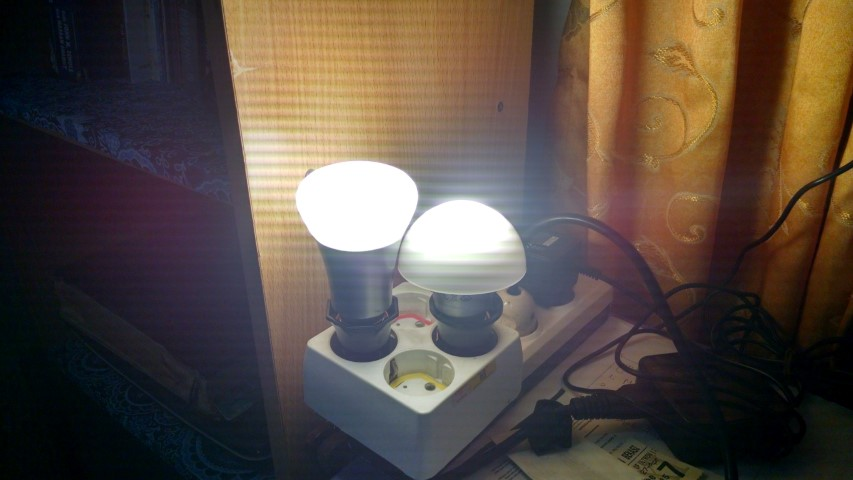
\includegraphics[width=.75\textwidth]{pics/uji23.jpg}\\
			\hline
			\textbf{Ekspektasi} & Kedua lampu menjadi lebih terang  \\
			\hline
		\end{tabular}
	\end{table}
	\item Kasus Uji 25: Mengubah warna lampu dalam suatu \textit{group} melalui pesan yang dikirimkan dari \textit{pub-sub system}.
	\begin{table}
		\centering
		\caption{Hasil pengujian kasus uji 25}
		\label{tab:kasusUji25}
		\begin{tabular}{| l | p{11cm} |}
			\hline
			\textbf{Topik} & \code{sot/g/557903af5ad821942ef0af51/ledlight /557d10c80fcf33af4e209d8e/hue/ctl}\\
			\hline
			\textbf{Prekondisi} & \textit{Group} sudah didaftarkan dengan atribut terkait diberikan hak kontrol, lampu anggota \textit{group} dalam keadaan menyala\\
			\hline
			\textbf{Isi pesan} & \code{65535}\\
			\hline
			\textbf{Hasil} & Kedua lampu menjadi berwarna merah
			
			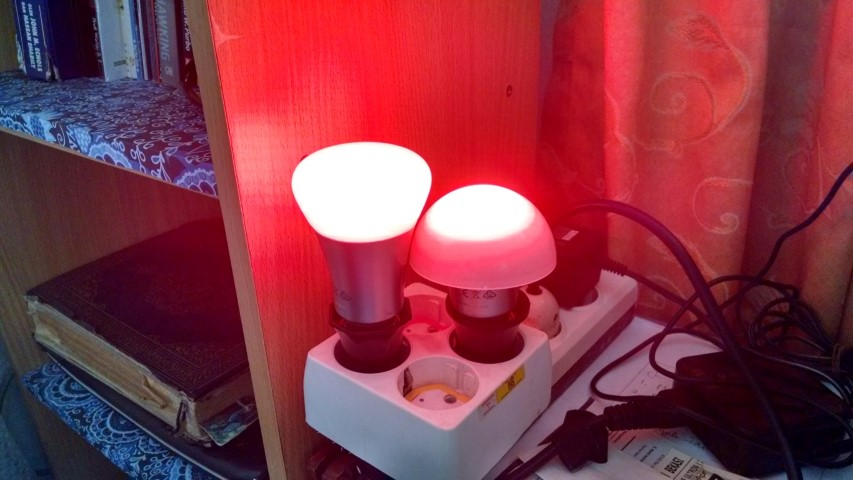
\includegraphics[width=.75\textwidth]{pics/uji24.jpg}\\
			\hline
			\textbf{Ekspektasi} & Kedua lampu menjadi berwarna merah  \\
			\hline
		\end{tabular}
	\end{table}
	\item Kasus Uji 26: Mengubah tingkat kejenuhan lampu dalam suatu \textit{group} melalui pesan yang dikirimkan dari \textit{pub-sub system}.
	\begin{table}
		\centering
		\caption{Hasil pengujian kasus uji 26}
		\label{tab:kasusUji26}
		\begin{tabular}{| l | p{11cm} |}
			\hline
			\textbf{Topik} & \code{sot/g/557903af5ad821942ef0af51/ledlight /557d10c80fcf33af4e209d8e/sat/ctl}\\
			\hline
			\textbf{Prekondisi} & \textit{Group} sudah didaftarkan dengan atribut terkait diberikan hak kontrol, lampu anggota \textit{group} dalam keadaan menyala\\
			\hline
			\textbf{Isi pesan} & \code{150}\\
			\hline
			\textbf{Hasil} & Kedua lampu menjadi berwarna lebih muda
			
			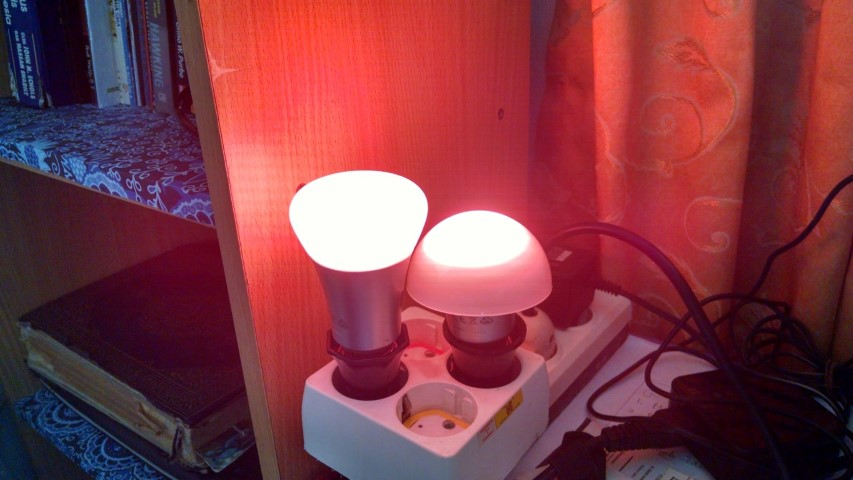
\includegraphics[width=.75\textwidth]{pics/uji25.jpg}\\
			\hline
			\textbf{Ekspektasi} & Kedua lampu menjadi berwarna lebih muda  \\
			\hline
		\end{tabular}
	\end{table}
\end{enumerate}
%-----------------------------------------------------------------------------%
\chapter{\babEnam}
%-----------------------------------------------------------------------------%
Pada bab ini dijelaskan mengenai hasil pengujian, kesimpulan dari implementasi perangkat \textit{gateway} yang telah dilakukan, serta saran dari \saya~untuk pengembangan selanjutnya.

\section{Hasil Pengujian}
Dari hasil pengujian, dapat dilihat bahwa perangkat \textit{gateway} sudah dapat beroperasi dan digunakan sesuai dengan tujuan. Perangkat \textit{gateway} dapat berperan sebagai sebuah \textit{access point} secara otomatis setelah perangkat dinyalakan. Perangkat \textit{gateway} juga kemudian dapat dihubungkan dengan \textit{access point} lainnya melalui halaman aplikasi web yang disediakan. Operasi untuk mengontrol lampu melalui halaman aplikasi web yang disediakan juga dapat dilakukan dengan sukses. Setelah terhubung ke internet, pengguna juga dapat mendaftarkan lampu atau \textit{group} ke \plat~dengan sukses. Perintah yang dikirimkan oleh \textit{pub-sub system} ke topik yang sesuai juga berhasil diterima dan dikerjakan dengan sukses. Terakhir, perangkat \textit{gateway} berhasil mengirimkan informasi mengenai kondisi setiap lampu atau \textit{group} terdaftar ke \textit{pub-sub system} setiap jangka waktu tertentu.

\section{Kesimpulan}
Dalam tugas akhir ini, \saya~berhasil menghubungkan sebuah jaringan lampu berbasis ZigBee dengan sebuah \textit{platform} \iot~berbasis media sosial. Dalam tugas akhir ini, digunakan Raspberry Pi sebagai perangkat untuk menjalankan semua operasi terkait sehingga tidak diperlukan lagi komputer tambahan. Berdasarkan implementasi yang telah dilakukan, \saya~dapat mengambil beberapa kesimpulan, yaitu:
\begin{enumerate}
	%\item Raspberry Pi dapat digunakan sebagai sebuah perangkat ZigBee \textit{gateway} dan menjalankan fungsinya dengan baik.
	%\item Perangkat \textit{gateway} yang dibuat dapat berkomunikasi dengan baik dengan \plat~yang ada dan dapat digunakan untuk mengendalikan jaringan lampu tanpa harus terhubung ke \plat.
	%\item Fungsi-fungsi untuk mengendalikan lampu dapat dilakukan melalui GUI dengan menggunakan API REST yang disediakan oleh deCONZ.
	%\item Penggunaan MQTT untuk mekanisme pengiriman pesan dari dan ke perangkat \textit{gateway} dapat berjalan dengan baik. Penggunaan topik MQTT membantu mempermudah proses implementasi sekaligus memberikan informasi yang dibutuhkan untuk membedakan banyak pengguna di dalam \plat. Dengan memberikan id pengguna pada topik, setiap perangkat \textit{gateway} dapat melakukan \textit{subscribe} hanya terhadap pesan yang relevan.
	\item Untuk membuat sebuah perangkat \textit{gateway} ZigBee berbasiskan GUI pada Raspberry Pi, diperlukan beberapa komponen. Komponen tersebut bisa diimplementasikan menggunakan \textit{tools} atau aplikasi yang telah tersedia. Komponen tersebut adalah:
	\begin{itemize}
	\item ZigBee \textit{coordinator} yang berfungsi untuk menghubungkan perangkat \textit{gateway} dengan perangkat ZigBee. Tools yang bisa digunakan adalah deCONZ yang disediakan oleh pihak Dresden Elektronik
	\item Sebuah kode implementasi \textit{gateway} yang bertugas menerjemahkan pesan dari dan ke koordinator. Kode ini bisa diimplementasikan menggunakan bahasa pemrograman Java dan dengan memodifikasi implementasi gateway yang telah dibuat oleh Fauziah Rahmawati\cite{SkripsiFarah}.
	\item \textit{Client} MQTT yang berfungsi sebagai \textit{publisher} dan \textit{subscriber}. \textit{Client} inilah yang akan menerima dan mengirim pesan ke \textit{platform} terkait. \textit{Tools} yang bisa digunakan adalah Paho yang disediakan oleh pihak Eclipse.
	\item Sebuah \textit{server database} lokal yang berfungsi menyimpan informasi terkait perangkat dan beberapa konfigurasi. \textit{Tools} yang bisa digunakan adalah MySQL.
	\item Sebuah \textit{web server} yang menjadi tempat untuk menjalankan aplikasi web berbasis GUI untuk diakses oleh pengguna. \textit{Tools} yang bisa digunakan adalah Apache.
	\end{itemize}
	
	\item Sebuah jaringan perangkat ZigBee dapat dihubungkan dengan \textit{social internet of things platform} berbasiskan media sosial dengan menggunakan konsep \textit{publish-subscribe} dengan tipe berdasarkan topik. Implementasi konsep \textit{publish-subscribe} ini dapat dilakukan menggunakan protokol MQTT.
	
	\item Perintah yang dikirimkan dari \textit{platform} melalui protokol MQTT diterjemahkan oleh \textit{gateway} dan disampaikan ke koordinator melalui REST API, dan informasi mengenai perangkat ZigBee akan diambil secara berkala dari koordinator dan kemudian dikirimkan ke \textit{platform} melalui protokol MQTT.
	
	\item Penggunaan konsep topik MQTT membantu mempermudah proses implementasi sekaligus memberikan informasi yang dibutuhkan untuk membedakan banyak pengguna di dalam \textit{platform}. Dengan memberikan id pengguna pada topik, setiap perangkat \textit{gateway} dapat melakukan \textit{subscribe} hanya terhadap pesan yang relevan. Selain membedakan antar pengguna, penggunaan konsep topik MQTT juga dapat digunakan untuk membedakan tiap atribut dalam satu perangkat.
\end{enumerate}

\section{Saran}
Setelah melakukan implementasi yang dijelaskan dalam tugas akhir ini, \saya~memiliki beberapa saran yang dapat digunakan untuk pengembangan sistem atau perangkat sejenis di masa depan:
\begin{enumerate}
	\item Implementasi \textit{coordinator} dapat dikembangkan sehingga dapat digunakan untuk mengontrol jenis perangkat ZigBee lainnya, seperti \textit{power outlet}, \textit{switch}, dan jenis perangkat dengan profil ZigBee lainnya.
	\item Implementasi perangkat \textit{gateway} untuk terhubung ke \textit{access point} masih dapat ditingkatkan. Sebagai contoh, untuk implementasi pada tugas akhir ini perangkat hanya bisa dihubungakan dengan \textit{access point} yang tidak menggunakan proteksi.
	\item Implementasi GUI untuk mengontrol lampu masih bisa ditingkatkan dalam hal \textit{user interface} dan \textit{user experience}.
	\item Perlu ditambahkan mekanisme otorisasi dalam pertukaran pesan menggunakan MQTT, sehingga pesan tidak bisa diakses oleh pengguna yang tidak berhak.
\end{enumerate}

%%---------------------------------------------------------------
\chapter{\kesimpulan}
%---------------------------------------------------------------
\todo{Tambahkan kesimpulan dan saran terkait dengan perkerjaan 
	yang dilakukan.}


%---------------------------------------------------------------
\section{Kesimpulan}
%---------------------------------------------------------------


%---------------------------------------------------------------
\section{Saran}
%---------------------------------------------------------------


%
% Daftar Pustaka
%%
% Daftar Pustaka 
% 

% 
% Tambahkan pustaka yang digunakan setelah perintah berikut. 
% 
\begin{thebibliography}{10}

\bibitem{1}
{Cisco. \f{The Internet of Things}.
Diakses 10 Maret 2015 \url{http://share.cisco.com/internet-of-things.html}.}

\bibitem{2}
{Nisrina Luthfiyati. \f{Implementasi zigbee \textit{coordinator} dengan REST \textit{interface}}.
Juni 2014.}

\bibitem{3}
{Fauziah Rahmawati. \f{"Implementasi \textit{Home Automation Gateway} untuk IOT \textit{Cloud Service} berbasis ZigBee \textit{Network}"}.
Januari 2015.}

\end{thebibliography}


\printbibliography

%
% Lampiran 
%
\begin{appendix}
	%
% @author  Andreas Febrian
% @version 1.00 
% 
% Hanya sebuah pembatas bertuliskan LAMPIRAN ditengah halaman. 
% 

\begin{titlepage}
	\centering 
	\vspace*{6cm}
	\noindent \Huge{LAMPIRAN}
	\addChapter{LAMPIRAN}
\end{titlepage}
	\setcounter{page}{2}
	%-----------------------------------------------------------------------------%
\addChapter{Lampiran 1}
\chapter*{Lampiran 1}
%-----------------------------------------------------------------------------%
\end{appendix}


\end{document}